\documentclass[12pt]{report}

\usepackage{styles/thesis_packages}


\usepackage{xspace}




% general astro conventions

\newcommand{\glon}{\text{GLON}\xspace}
\newcommand{\glat}{\text{GLAT}\xspace}


% neutron star

\newcommand{\MassChandrasekhar}{\ensuremath{\Mass_\text{Ch}}\xspace}
\newcommand{\MassNeutronStar}{\ensuremath{\Mass_\text{ns}}\xspace}
\newcommand{\RadiusNeutronStar}{\ensuremath{R_\text{ns}}\xspace}

% pulsar
\newcommand{\energyrotational}{\ensuremath{\energy_\text{rot}}\xspace}

\newcommand{\PulsarRotationAngle}{\ensuremath{\theta}\xspace}
\newcommand{\PulsarRadius}{\ensuremath{R_\text{NS}}\xspace}

\newcommand{\period}{\ensuremath{P}\xspace}
\newcommand{\perioddot}{\ensuremath{\dot{\period}}\xspace}
\newcommand{\perioddotdot}{\ensuremath{\ddot{\period}}\xspace}

\newcommand{\PulsarAngularFrequency}{\ensuremath{\Omega}\xspace}
\newcommand{\PulsarAngularFrequencyDot}{\ensuremath{\dot{\PulsarAngularFrequency}}\xspace}
\newcommand{\PulsarAngularFrequencyDotDot}{\ensuremath{\ddot{\PulsarAngularFrequency}}\xspace}


\newcommand{\frequency}{\ensuremath{\nu}\xspace}
\newcommand{\angularfrequency}{\ensuremath{\omega}\xspace}

\newcommand{\breakingindex}{\ensuremath{n}\xspace}
\newcommand{\SpinDownTimescale}{\ensuremath{\tau_\text{dec}}\xspace}

\newcommand{\momentofinertia}{\ensuremath{I}\xspace}
\newcommand{\lifetime}{\ensuremath{\tau}\xspace}
\newcommand{\PulsarAge}{\ensuremath{\tau_c}\xspace}

\newcommand{\PulsarPotential}{\ensuremath{\Delta \Phi}\xspace}

\newcommand{\solarmass}{\ensuremath{\Mass_{\odot}}\xspace}

% pwn stuff

\newcommand{\radiusterminationshock}{\ensuremath{r_\text{ts}}\xspace}
\newcommand{\pointingflux}{\ensuremath{F_{E\times B}}\xspace}
\newcommand{\particleflux}{\ensuremath{F_\text{particle}}\xspace}
\newcommand{\magnetization}{\ensuremath{\sigma}\xspace}

\newcommand{\pressureISM}{\ensuremath{P_\text{ISM}}\xspace}


\newcommand{\KleinNishinaCrossSection}{\ensuremath{\CrossSection_\text{KN}}\xspace}

\newcommand{\pion}{\ensuremath{{\pi}^0}\xspace}

\newcommand{\luminosity}{\ensuremath{L}\xspace}


\newcommand{\prefactor}{\ensuremath{N_0}\xspace}
\newcommand{\spectralindex}{\ensuremath{\gamma}\xspace}
\newcommand{\Escale}{\ensuremath{E_0}\xspace}

\newcommand{\Ecutoff}{\ensuremath{E_c}\xspace}
\newcommand{\Ebreak}{\ensuremath{E_b}\xspace}


% Names of Experiments
\newcommand{\explorerxi}{Explorer XI\xspace}
\newcommand{\fermi}{\textit{Fermi}\xspace}
\newcommand{\cosb}{COS-B\xspace}

\newcommand{\chandra}{\text{{\em Chandra}}\xspace}
\newcommand{\swiftxrt}{\text{{\em Swift}/XRT}\xspace}
\newcommand{\rosat}{\text{{\em ROSAT}}\xspace}
\newcommand{\suzaku}{\text{{\em Suzaku}}\xspace}
\newcommand{\asca}{\text{{\em ASCA}}\xspace}
\newcommand{\einstein}{\text{{\em Einstein}}\xspace}
\newcommand{\xmmnewton}{\text{{\em XMM-Newton}}\xspace}

\newcommand{\tevcat}{\text{TeVCat}\xspace}

% Fermi Tools
\newcommand{\pointlike}{\ensuremath{\mathtt{pointlike}}\xspace}
\newcommand{\gtlike}{\ensuremath{\mathtt{gtlike}}\xspace}
\newcommand{\gtobssim}{\ensuremath{\mathtt{gtobssim}}\xspace}
\newcommand{\gtselect}{\ensuremath{\mathtt{gtselect}}\xspace}
\newcommand{\gtbin}{\ensuremath{\mathtt{gtbin}}\xspace}
\newcommand{\gtltcube}{\ensuremath{\mathtt{gtltcube}}\xspace}
\newcommand{\gtexpcubetwo}{\ensuremath{\mathtt{gtexpcube2}}\xspace}
\newcommand{\gtsrcmaps}{\ensuremath{\mathtt{gtsrcmaps}}\xspace}

\newcommand{\fits}{\ensuremath{\mathtt{fits}}\xspace}

\newcommand{\tsextpointlike}{\ensuremath{{\tsext}_{,\pointlike}}\xspace}
\newcommand{\tsextgtlike}{\ensuremath{{\tsext}_{,\gtlike}}\xspace}
\newcommand{\tsextaltdiff}{\ensuremath{{\tsext}_{\altdiff}}\xspace}

\newcommand{\tstev}{\ensuremath{\ts_\tev}\xspace}
\newcommand{\tspointlike}{\ensuremath{\ts_{\pointlike}}\xspace}
\newcommand{\tsgtlike}{\ensuremath{\ts_{\gtlike}}\xspace}
\newcommand{\tsaltdiff}{\ensuremath{\ts_{\altdiff}}\xspace}

\newcommand{\altdiff}{\text{alt,diff}\xspace}
\newcommand{\altpsf}{\text{alt,psf}\xspace}


% Detector commands
\newcommand{\modelparams}{\ensuremath{\myvector{\lambda}}\xspace}
\newcommand{\fluxdensity}{\mathcal{F}\xspace}
\newcommand{\effectivearea}{\ensuremath{\epsilon}\xspace}
\newcommand{\dispersion}{\ensuremath{P}\xspace}
\newcommand{\response}{\ensuremath{R}\xspace}
\newcommand{\eventrate}{\ensuremath{\tau}\xspace}
\newcommand{\psf}{\ensuremath{\text{PSF}}\xspace}
\newcommand{\edisp}{\ensuremath{\text{E}_\text{disp}}\xspace}
\newcommand{\tdisp}{\ensuremath{\text{T}_\text{disp}}\xspace}

\newcommand{\dnde}{\ensuremath{\frac{dN}{d\energy}}\xspace}

% Other fermi stuff
\newcommand{\psevensourcevsix}{\texttt{P7SOURCE\_V6}\xspace}
\newcommand{\galprop}{\texttt{GALPROP}\xspace}
\newcommand{\healpix}{\texttt{HEALPIX}\xspace}

% paper referencing
\newcommand{\paperref}[1]{\begin{quote}\em{#1}\end{quote}}

% References
\newcommand{\chapref}[1]{Chapter~\ref{chap:#1}}
\newcommand{\secref}[1]{Section~\ref{sec:#1}}
\newcommand{\subsecref}[1]{Section~\ref{subsec:#1}}
\newcommand{\tabref}[1]{Table~\ref{tab:#1}}
\newcommand{\figref}[1]{Figure~\ref{fig:#1}}
\newcommand{\eqnref}[1]{Equation~\ref{eqn:#1}}

% Labeling
\newcommand{\chaplabel}[1]{\label{chap:#1}}
\newcommand{\seclabel}[1]{\label{sec:#1}}
\newcommand{\subseclabel}[1]{\label{subsec:#1}}
\newcommand{\tablabel}[1]{\label{tab:#1}}
\newcommand{\figlabel}[1]{\label{fig:#1}}
\newcommand{\eqnlabel}[1]{\label{eqn:#1}}



% pulsar
\newcommand{\energydot}{\ensuremath{\dot{\energy}}\xspace}

\newcommand{\period}{\ensuremath{P}\xspace}
\newcommand{\perioddot}{\ensuremath{\dot{\period}}\xspace}

% characteristic pulsar age
\newcommand{\momentofinertia}{\ensuremath{I}\xspace}
\newcommand{\pulsarage}{\ensuremath{\tau_c}\xspace}


% fermi sources

\newcommand{\velax}{Vela~X\xspace}

\newcommand{\twofgl}[2]{2FGL$\,$J$#1#2$\xspace}


% spacing between units and numbers, i.e. 100\unitspace\mev
\newcommand{\unitspace}{\,}

% Units
\newcommand{\ph}{\text{ph}\xspace}
\newcommand{\erg}{\text{erg}\xspace}

\newcommand{\cm}{\text{cm}\xspace}
\newcommand{\km}{\text{km}\xspace}
\newcommand{\parsec}{\text{pc}\xspace}
\newcommand{\kiloparsec}{\text{kpc}\xspace}


\newcommand{\gauss}{\text{G}\xspace}

\newcommand{\gram}{\text{g}\xspace}
\newcommand{\second}{\text{s}\xspace}
\newcommand{\steradian}{\ensuremath{\text{sr}}\xspace}

\newcommand{\electronvolt}{\ensuremath{\text{eV}}\xspace}
\newcommand{\mev}{\ensuremath{\text{MeV}}\xspace}
\newcommand{\gev}{\ensuremath{\text{GeV}}\xspace}
\newcommand{\tev}{\text{TeV}\xspace}
\newcommand{\fluxunits}{\ensuremath{\ph\;\cm^{-2}\second^{-1}}\xspace}
\newcommand{\efluxunits}{\ensuremath{\erg\;\cm^{-2}\second^{-1}}\xspace}
\newcommand{\prefunits}{\ensuremath{\fluxunits\erg^{-1}}\xspace}

\newcommand{\fluxdensityunits}{\ensuremath{\prefunits\steradian^{-1}}\xspace}

\newcommand{\pdfunits}{\ensuremath{\steradian^{-1}}\xspace}

\newcommand{\microsecond}{\ensuremath{\mu\text{s}}\xspace}

\newcommand{\absval}[1]{\ensuremath{|#1|}}

% space between terms in integral
\newcommand{\intspace}{\;}

\newcommand{\derivative}{\ensuremath{\text{d}}\xspace}

\newcommand{\solidangle}{\ensuremath{\vec\Omega}\xspace}
\newcommand{\dsolidangle}{\ensuremath{d\Omega}\xspace}

\newcommand{\degree}{\ensuremath{^\circ}\xspace}

% Note, these commands come from aastex.cls
\newcommand\arcsec{\mbox{$^{\prime\prime}$}}%
\newcommand\fdg{\mbox{$.\!\!^\circ$}}%
\newcommand\arcmin{\mbox{$^\prime$}}%


% vector operations
\newcommand{\myvector}[1]{\ensuremath{\boldsymbol{#1}}\xspace}

\newcommand{\cross}[2]{\ensuremath{#1\!\boldsymbol{\times}\!#2}}

\newcommand{\minuit}{\ensuremath{\mathtt{minuit}}\xspace}


% Likelihood analysis stuff
\newcommand{\likelihood}{\mathcal{L}\xspace}
\newcommand{\data}{\ensuremath{\text{data}}\xspace}
\newcommand{\model}{\ensuremath{\text{model}}\xspace}
\newcommand{\pdf}{\ensuremath{\text{PDF}}\xspace}

\newcommand{\ts}{\mathrm{TS}\xspace}
\newcommand{\tspoint}{\ts_\mathrm{point}\xspace}
\newcommand{\tsext}{\ensuremath{\ts_\mathrm{ext}}\xspace}
\newcommand{\tscutoff}{\ensuremath{\ts_\mathrm{cutoff}}\xspace}
\newcommand{\Ecutoff}{\ensuremath{E_\mathrm{cutoff}}\xspace}
\newcommand{\tsvar}{\ensuremath{\ts_\mathrm{var}}\xspace}




%nat This prevents commas between authors and years with natbib
\citestyle{aa}



\title{Observations of PWNe with the Fermi Gamma-ray Space Telescope}
\author{Joshua Jeremy Lande}
\dept{Physics}
\principaladviser{Stefan Funk}
\firstreader{Elliott Bloom}
\secondreader{Roger Romani}


%the following command would (if uncommented) allow  only chapter1 and
%chapter2 to be processed
%\includeonly{chapter1,chapter2}

\begin{document}


% VVVVVVV THIS SHOULD EVENTUALLY BE REMOVE VVVVVVV
\listoftodos
\newpage
% ^^^^^^^ THIS SHOULD EVENTUALLY BE REMOVE ^^^^^^^ 
 

% first the preface sections.  

% this includes the file preface.tex which should include the
% following commands
\beforepreface
\prefacesection{Abstract}

\begin{quote}
\em{Two things fill the mind with ever-increasing wonder and awe,
the more often and the more intensely the mind of thought is drawn to
them: the starry heavens above me and the moral law within me.'' -- Immanuel Kant}
\end{quote}

The launch of the \fermi Gamma-ray space telescope in 2008 offered
an unprecedented view into the $\gamma$-ray sky.

All the things we can learn with the \gls{LAT}

Development of a new analysis method for studying spatially-extended \glspl{PWN}
using \pointlike.

A monte-carlo validation of the analysis method.

Search for new spatially-extended sources with the \gls{LAT}.

Observations of \glspl{PWN} in the off-peak region of \gls{LAT} detected pulsars.

Search for \glspl{PWN} counterparts to TeV sources.

Using the population of \glspl{PWN} to understand the radiation mechanism of \glspl{PWN}.


\prefacesection{Acknowledgement}

Acknowkege the educational institutes which taught me physics: My high school HB Woodlawn,
my undergraduate institution Marlboro College, and my Stanford University.

First, I would like to acknowlege those mentors who inspired me to get a PhD.
\begin{itemize}
  \item Mark Dodge, my high school physics teacher.
  \item Ron Turner, my internship adviser at Analytic Services (ANSER) during the 
  GWU Science and Engineering Apprentice Program (SEAP)
  \item Anthony Tyson at UC Davis for my SULI Internship
  \item Apurva Mehta and Sam Webb sam Web at SLAC SULI Internship.
\end{itemize}


During my PhD I was helped by an almost overwhelminlgy large 
number of people in the \gls{LAT} collaboration.

People at Stanford/SLAC: Stefan Funk, Elliott Bloom, 
Markus Ackermann, Tobias Jogler, Junichiro Katsuta, Yasunobu Uchiyama, Seth Digel, 
James Chiang

\pointlike collaborators: Matthew Kerr, Toby Burnett, Eric Wallace, Marshall Roth

Pulsar Collaborators: David Smith, Matthew Kerr, Peter den Hartog, Tyrel Johnson, Damien Parent, Ozlem Celik

Careful review of text: Jean Ballet, Johann Cohen-Tanugi

I would like to thank the \glspl{PWN} people
Thank the people in Bordeaux: Marianne Lemoine-Goumard, Romain Rousseau, and Marie-H\'el\`ene Grondin


Fermi SLAC Grad Students: Keith Bechtol, Alex Drlica-Wagner, Alice Allafort, Herman Lee
Yvonne Edmonds, Bijan Berenji, Ping Wang, Warit Mitthumsiri


Joanne Bogart, Heather Kelly, Richard Dubois, Renata Dart, Stuart Marshall, and Glenn Morris for putting up with my computer problems.

Martha Siegel, Chris Hall, Ziba Mahdavi, awesome SLAC administrators.
Maria Frank, Elva Carbajal, and Violet Catindig , awesome Stanford administrators.

Additional Astro Stanford Graduate Students: Helen Craig, Michael Shaw, Adam Van Etten, Kyle Watters

Additonal Graduate Students at Stanford: Dan Riley, Joel Frederico, Ahmed Ismail, Joshua Cogan, Kunal Sahasrabuddhe,

\afterpreface

% Note, we had to override the acronyms a little bit to allow some
% customization.
% Following the discussion from https://groups.google.com/d/msg/comp.text.tex/_NBZd1p8g8Q/X9QOZID_wm4J
% now:
%  * user1=stores the indefinite article for the expanded version
%  * user2=stores the indefinite article for the abbreviation version
%  * user3=The expanded acronym in title case
%  * user4=The expanded plural acronym in title case.
%
% The defaults are: user1='a', user2='a', 
% user3='the expanded title (not title case),
% user4='the expanded title (not title case & not plural),

% We defined the new commands:
%  * \agls: puts the indefinite article in front of the acronym 
%    e.g. "an IDN" or "a identification number (IDN)"
%  * \Agls: same as \agls, but in upper case
%    e.g. "An IDN" or "A identification number (IDN)"
%  * \Actitle: writes out the title in full
%    e.g. "Pulsar Wind Nebula"
%  * \Acptitle: writes out the plural title in full
%    e.g. "Pulsar Wind Nebulae"


\newcommand{\mynewacronym}[4][]{%
   \newacronym[user1=a,user2=a,user3=#4,user4=#4, #1]{#2}{#3}{#4}}

\newcommand{\agls}[1]{%
   \ifglsused{#1}{\glsentryuserii{#1}}{\glsentryuseri{#1}}
   \gls{#1}%
}

\newcommand{\Agls}[1]{%
   \ifglsused{#1}{\Glsentryuserii{#1}}{\Glsentryuseri{#1}}
   \gls{#1}%
}

\newcommand{\Actitle}[1]{\glsentryuseriii{#1}}
\newcommand{\Acptitle}[1]{\glsentryuseriv{#1}}

%%%%%%%%%%%%%%%%%%%%%%%%%%%%%%%%%%%%%%%%%%%%%%%%%%%%%%%%%%%%%%%%%%%%%%%%%%%

% Math stuff

\mynewacronym{SA}{SA}{solid angle}
\mynewacronym{FWHM}{FWHM}{full width at half maximum}

% Fermi Stuff

\mynewacronym{LAT}{LAT}{the Large Area Telescope}


\mynewacronym{ACD}{ACD}{Anti-Coincidence Detector}
\mynewacronym{GBM}{GBM}{Gamma-ray Burst Monitor}

% Astrophysical sources

\mynewacronym[longplural=pulsar wind nebulae,
            shortplural=PWNe,
            user3=Pulsr Wind Nebula,
            user4=Pulsar Wind Nebulae]{PWN}{PWN}{pulsar wind nebula}
\mynewacronym{SNR}{SNR}{supernova remnant}
\mynewacronym{NS}{NS}{neutron star}
\mynewacronym{MSP}{MSP}{millisecond pulsar}

% radiation mechanisms
\mynewacronym{IC}{IC}{inverse Compoton}

% catalogs
\mynewacronym{2CG}{2CG}{the second \cosb catalog}
\mynewacronym[user3=The Second Fermi Catalog]{2FGL}{2FGL}{the second \fermi catalog}
\mynewacronym[user3=The Second Fermi Pulsar Catalog]{2PC}{2PC}{the second \fermi pulsar catalog}
\mynewacronym{3EG}{3EG}{the Third EGRET Catalog}

% math stuff
\mynewacronym{CGS}{CGS}{the Centimetre-Gram-Second System of Units}

% source models
\mynewacronym{PL}{PL}{power law}
\mynewacronym{ECPL}{ECPL}{exponentially-cutoff power law}
\mynewacronym{BPL}{BPL}{broken-power law}

% schools
\mynewacronym{MIT}{MIT}{the Massachusetts Institute of Technology}

% experiments
\mynewacronym{OSO-3}{OSO-3}{the Third Orbiting Solar Observatory}
\mynewacronym{SAS-2}{SAS-2}{the second Small Astronomy Satellite}
\mynewacronym{EGRET}{EGRET}{the Energetic Gamma Ray Experiment Telescope}
\mynewacronym{CGRO}{CGRO}{the Compton Gamma Ray Observatory}

% Goverment Stuff
\mynewacronym{ESA}{ESA}{the European Space Agency}
\mynewacronym{NASA}{NASA}{the National Aeronautics and Space Administration}
\mynewacronym{NRL}{NRL}{the Naval Research Laboratory}

\mynewacronym[longplural=seconds of arc,shortplural=arcsecs]{arcsec}{arcsec}{second of arc}


% now for the body of the thesis, modify the number of these lines as needed

% Reset the acronym counts in the main text
\acresetall

\chapter{Overview}

In \chapref{gamma_ray_astro}, we discuss the history of $\gamma$-ray
astrophysics. First we present broadly the history of astronomy in
\secref{astronomy_and_the_atmosphere} and the history of $\gamma$-ray
astrophysics in \secref{history_gamma_ray_detectors}.  Then, we discuss
the \fermi Gamma-ray Space Telescope in \secref{fermi_telescope}.  Next,
we discuss historical developments in our understanding of pulsars and
\ac{PWN} in \secref{pulsars_and_pwn}.  We conclude by discussing the major
source classes detected by the \ac{LAT} in \secref{sources_detected_fermi}
adn the major radiation processes that occur in high-energy astrophysics
in \secref{radiation_processes}.

In \chapref{pulsar_pwn_system}, we discuss our current understanding
of the physics of pulsars and \ac{PWN}.  We discuss the formation of a
pulsar in \secref{neutron_star_formation} and the time evolution of a
pulsar in \secref{pulsar_evolution}.  Then, we describe the magnetosphere
of the pulsar in \secref{pulsar_magnetosphere} and the structure of a
typical \ac{PWN} in \secref{pwn_structure}.  Finally, we describe the
energy spectrum emitted from a typical \ac{PWN} in \secref{pwn_emission}.

In \chapref{maximum_likelihood_analysis}, we discuss maximum-likelihood
analysis and how it can be used to analyze \ac{LAT} data.
We describe the motivation for using maximum-likelihood analysis
in \secref{motivations_maximum_likelihood}
and the maximum-likelihood formulation in
\secref{description_maximum_likelihood}.  Then, we describe how to build
a model of the $\gamma$-ray sky in \secref{defining_model} and describe
the \ac{LAT} \acp{IRF} in \secref{lat_irfs}.
Finally, 
we describe the standard
package \gtlike for performing maximum-likelihood analysis of \ac{LAT}
data in \secref{binned_science_tools} and we describe \pointlike,
an alternate package for performing maximum-likelihood analysis of
\ac{LAT} data, in \secref{pointlike_package}.

In \chapref{extended_analysis}, we discuss a new method to study
spatially-extended sources.  We discuss the formulation of this
method in \secref{analysis_methods_section}.  We validate the
extension-significance calculation in \secref{validate_ts} and then
we compute the sensitivity of the \ac{LAT} to spatially-extended
sources in \secref{extension_sensitivity}.  We develop a new method
to compare the hypothesis of multiple point-like sources to one
spatially-extended source in \secref{dual_localization_method} and
finally in \secref{test_2lac_sources} we validate our method by testing
point-like sources from \ac{2LAC} for extension.

In \chapref{extended_search}, we apply the extension test developed in
\chapref{extended_analysis} to search for new spatially-extended sources.
First, we validate the method by studying known spatially-extended
\ac{LAT} sources in \secref{validate_known}.  

In \secref{systematic_errors_on_extension}, we develop a method
to estimate systematic errors associated with studying extended
sources and in \secref{extended_source_search_method} we develop
a method to search for new spatially-extended sources.  Finally,
we discuss the newly-discovered spatially-extended sources in
\secref{new_ext_srcs_section} and the population of spatially-extended
\ac{LAT} sources in \secref{extended_source_discussion}.

In \chapref{offpeak}, we perform a search for new \ac{PWN} in the
off-peak regions of \ac{LAT}-detected pulsars.  First, we develop
a new method to define the off-peak regions used for the search in
\secref{peak_definition}.  Then, we describe the analysis method we
used to search these regions in \secref{off_peak_analysis} and the
results of this search in \secref{off_peak_results}.  Finally,
we discuss some of the sources detected with this method in
\secref{off_peak_individual_source_discussion}.

In \chapref{tevcat}, we perform a search for $\gamma$-ray emission
from \ac{VHE} \ac{PWN}.  We discuss our list of \ac{VHE} candidates
in \secref{tevcat_list_vhe_pwn_candidates} and our analysis method
in \secref{tevcat_analysis_method}.  Finally, we several new \ac{PWN}
detected using this method in \secref{tevcat_sources_detected}.

In \chapref{population_study}, we describe the population of $\gamma$-ray
emitting \ac{PWN} and study how they evolve with the spin-down energy
and age of their associated pulsars.  Finally, in \chapref{outlook} we
remark on potential future opportunities to expand our understanding of
\acp{PWN} and their $\gamma$-ray emission.



\chapter{Introduction}

\section{Gamma-ray Detectors}
\subsection{The \fermi Gamma-ray Space Telescope}
\subsection{H.E.S.S.}

\section{Galactic Gamma-ray Astrophysics}
\subsection{Pulsars}
\subsection{Pulsar Wind Nebulae}
\subsection{Supernova Remenants}

\section{Radiation Processes}

\begin{itemize}
  \item The non-thermal radiation processes typical
    in astrophysics are most comonly
\end{itemize}

\subsection{Synchrotron}

\subsection{Inverse Compton}

\subsection{Bremsstrahlung}

\subsection{Pi0 Decay}

\section{Modeling the Galactic Diffuse and Isotropic Gamma-ray Background}
\seclabel{modeling_background}

\begin{itemize}
  \item Historical Observations of galactic diffuse emission
  \item GALPROP model of diffuse emission.
  Reference: \url{http://arxiv.org/abs/1202.4039}
  \item Emperical Ring model of galactic diffuse emisson.
  \item The isotropic background: \url{http://arxiv.org/abs/1002.3603}
\end{itemize}

\begin{itemize}
  \item Galactic diffuse emission is primarily composed of \ldots
  \item Something about how great galprop is.
  \item Something about
\end{itemize}

\section{Sources Detected by the Fermi LAT}

\begin{itemize}
  \item A variety of sources detected by the LAT:
\end{itemize}

\subsection{The Second Fermi-LAT Source Catalog}

\begin{itemize}
  \item Citation is \cite{second_lat_catalog_2012}
  \item Source classification method
  \item Number of sources detected by the LAT
  \item Forward reference \chapref{maximum_likelihood_analysis},
    which does a more thorough description of likelihood analysis method.
  \item Source classes/associations
\end{itemize}

\subsection{The Second Fermi Pulsar Catalog}

\begin{itemize}
  \item Process of detecting Pulsars with the LAT
  \item Number of pulsars detected by the LAT
\end{itemize}

\subsection{PWN Detected by the LAT}

\subsubsection{Crab}

\subsubsection{Vela X}

\subsubsection{MSH 15-52}

\subsubsection{HESS J1825}

\subsubsection{HESS J1857}

\twofgl{1857}{+026}

\begin{enumerate}
  \item Reference is \cite{hess_j1857_lat_2012}
  \item \url{http://arxiv.org/pdf/1206.3324v1.pdf}
\end{enumerate}


\chapter{Maximum-likelihood analysis of LAT data}
\chaplabel{maximum_likelihood_analysis}

\begin{itemize}
  \item The notation and terminology in this section 
    is primarily taken from \cite{matthew_kerr_thesis}.
\end{itemize}

\section{Motivations for Maximum-Likelihood Analysis of Gamma-ray Data}
\seclabel{motivations_maximum_likelihood}

Traditonally, spectral and spatial analysis of astrophysical data
relies on a process known as aperture photometry.  In this process,
a source in the data is analyzed by directly measuring the number of
photons coming from the object. This process is done by measuring the
counts within a given radius of the source and subtracting from it a
background level estimated from a nearby region.  Often, the source's
flux is calibrated by measurements of nearby objects with known fluxes.
Otherwise, the flux can be obtained from by dividing the number of
counts from the source by the telesocpe's size, the observation time,
and the telescope's conversion efficiency.

Similarly, for faint sources the statistical significance of the
detection can be obtained from the Poission nature of the data. For
TeV experiments such as H.E.S.S., this analysis method is described in
\cite{li_1983_analysis-methods}.

Unfortunately, this simpler analysis method is inadequate for dealing
with the complexities introduced in analyzing LAT data.  

Most importantly, aperture photometry assumed that the
background is istropic so that the background level below the source
can be estimated from nearby regions.
As was discussed in \secref{modeling_background},
the Galactic diffuse emission is highly anistropic,
rendering this assumption invalid.


% Note, number of square degrees in whole sky is 
%  * solid angle = 4*pi(180/pi)^2 = 129600/pi ~ 41,253 deg^2
%  * sqrt(41253 deg^2/1873) = 4.69 deg ~ 

% Command to find number of sources with LAT<=5degrees
% >>> import pyfits as pf,numpy as np
% >>> x=pf.open("gll_psc_v07.fit")[1].data;
% >>> lon,lat=x["GLON"],x["GLAT"]
% >>> cut=(np.abs(lat)<=0.5)&((lon<=0+45)|(lon>=360-45))
% >>> print np.sum(cut),len(cut)
% ... 73 1873

% Approximate Solid angle of plane ~ 90deg * 1deg = 90 deg^2

In addition,
this method is not optimal due to the high density of sources
detected in the Gamma-ray sky.  \ac{2FGL} reported on the detection
of 1873 sources, which corresponds to an average source spacing of
$\sim5\degree$.  But within the inner $45\degree$ of the galactic plane
in longitude and $0.5\degree$ of the galactic plane in latitidue, there
are 73 sources, corresponding to a source density of $\sim 1$ source per
square degree.  The aperature photometry method is unable to effecitvly
fit multiple sources when the tails of the PSF overlap and furthermore
make background estimation problematic.

Finally, this method is suboptimal due to the large energy range of
LAT observations.  A typical spectral analysis studies a source from
an energy of 100 \mev to energies above 100 \gev.  Similarly, as was
shown in \todo{what section discusses energy dependent psf?}, the PSF
of the LAT is rather broad ($\gtrsim 1\degree$) at low energy and much
narrower ($\sim 0.1\degree$) at higher energies. Therefore, there is a
much higher sensitivty to the higher energy photons coming from a source.
But simple aperture photometry method would ignore this improvement by
weighting each photon equally.



\section{Defining a Model of the Sources in the Sky}
\seclabel{defining_model}

\begin{itemize}
  \item
% THis notation is roughly taken from page 23 of Matthew Kerr's Thesis.
% with some parts adapted from 
%   http://www-glast.slac.stanford.edu/software/datachallenges/dc2/JuneWorkshop/Downloads/Likelihood_performance.pdf
Each source can be characterized by its photon flux density 
  $\fluxdensity(\energy,\time,\vec\Omega|\modelparams)$.
This is the number of photons emitted per unit energy, time, into a unit solid angle $d\Omega$
at a given energy, time, and position $\vec\Omega$ in the sky.

\item Typically, spatial and spectral model's are indepndent of time
  with the spatial and spectral component decopuling:
  \begin{equation}
    \fluxdensity(\energy,\time,\vec\Omega|\modelparams) = A(E) B(\vec\Omega)
  \end{equation}
  Presumably, $A$ takes in some of the \modelparams parameters
  and $B$ takes in the other parameters.
\item In situations where there is a time dependence, likelihoood assuming constant
  source is performed in smaller time bins.
\item In situations where spatial and spectral components couple, typical to make
  multiple spatial templates, each with an indepdnet spectra (e.g. the Puppis A paper's
  fitting multiple hemispheres).
\item Discuss how diffuse background is more complciated.
\item Show some examples spectral models: point source, extended source.
\end{itemize}


\section{The LAT Instrument Response Functions}


The performance of the LAT is composted of two effects.
The efficiency of the LAT referes to its ability to to
reconstruct a photon which comes into the detect.
The disperson of the LAT refers to the probability of
misreconstructing an event. 

The efficiency is typically called the effective area.
We write it as $\effectivearea(\energy,\time,\solidangle)$ 
and measure it in units of area ($\cm^2$).

\todo[inline]{LINK TO arXiv:1206.1896 for MORE THOUROUGH
DISCUSSION OF EFFECTIVE AREA}

\todo[inline]{DISCUSS HOW EFFECTIVE AREA IS A FUNCTION OF DIFFERENT THINGS}

The dispersion is the probability of a photon with true energy \energy
and incoming direction $\solidangle$ at time \time being reconstructed to 
to have an energy $\energy'$, an incomming direction $\solidangle'$ at a time $\time'$.
The dispersion is written as $\dispersion(\energy',\time',\solidangle'|\energy,\time,\solidangle)$.
It represents a probability and is therefore normalized such that
\begin{equation}
  \int \int \int \denergy \dsolidangle \dtime \dispersion(\energy',\time',\solidangle'|\energy,\time,\solidangle) = 1
\end{equation}
\todo[inline]{What is the range of the integrals}
Therefore, $\dispersion(\energy',\time',\solidangle'|\energy,\time,\solidangle)$ 
has units of 1/energy/solid angle/time

%We further break the diseprsion into two components, once associated with the
%spatial 

%\todo[inline]{What about temporal dispersion}

We assume these two factors to decouple and write the LAT's instrument response as
\begin{equation}
  \response(\energy',\solidangle',\time'|\energy,\solidangle,\time) = 
\effectivearea(\energy,\time,\solidangle) \dispersion(\energy',\time',\solidangle'|\energy,\time,\solidangle)
\end{equation}
Therefore, the instrument response has units of area/energy/solid angle/time

The convolution of the flux of a model with the instrument response 
produces the expected counts per unit energy/time/solid angle
begin reconstructed to have 
an energy $\energy'$ 
at a position $\solidangle'$ and at a time $\time'$:
\begin{equation}
  \eqnlabel{eventrate}
  \eventrate(\energy',\solidangle',\time'|\modelparams)
  = \int \int \int \denergy \, \dsolidangle \, \dtime \,
  \fluxdensity(\energy,\time,\vec\Omega|\modelparams) \response(\energy',\solidangle',\time'|\energy,\solidangle,\time)
\end{equation}
Here, this integral is performed over all true energies, solid angles, and times
for which the source model has support.

For LAT analysis, we conventionally make the simplifying assumption that
the energy , spatial , and time dispersion decouple:
\begin{equation}
  \dispersion(\energy',\time',\solidangle'|\energy,\time,\solidangle) = 
  \psf(\solidangle'|E,\solidangle) \times \edisp(\energy'|\energy) \times \tdisp(\time'|\time)
\end{equation}

Here, \psf is the point-spread function and represents 

% Information from section 7.1.3 of Eric Charles' calibration paper (arXiv:1206.1896)
\edisp represents the energy dispersion of the LAT.
The energy dispersion of the LAT is a function of both the
incident energy and incident angle of the photon. It varies
from $\sim$ 5\% to 20\%, degrading at lower energies due to energy
losses in the tracker and at higher energy due to electromagnetic
shower losses outside the calorimiter. Similarly, it improves
for photons with higher incident angles that are 
allowed a longer path through the calorimieter \citep{lat_calibration_2012}.

% This information comes from seciton 7.4 of Eric Charles' calibration paper (arXiv:1206.1896)
For sources with smoothly-varying spectra, the effects of ignoring
the inherent energy dispersion of the LAT are typically small.
\cite{lat_calibration_2012} performed a monte carlo simulation to show
that for power-law point-like sources, the bias introduced by ignoring
energy dispersion was on the level of a few perect.  Therefore, energy
dispersion is typicially ignored for standard likelihood analysis:
\begin{equation}
\edisp = \delta(\energy-\energy')
\end{equation}
We cauation that for analysis of sources extended to energies below 100
MeV and for sources expected to have spectra that do not smoothly vary,
the effects of energy dispersion could be more severe.

\begin{itemize}
  \item \tdisp is the time dispersion. 
  \item \todo{Why discard time dispersion}
  \item The timing dispersion is $<10$ \microsecond\cite{lat_mission_atwood_2009}
\item \todo[inline]{WRITE ENERGY DISPERSION AS A DELTA FUNCTION}
\end{itemize}

\todo{FINISH}
Therefore, the instrument response is typically approximated as
\begin{equation}
  \response(\energy',\solidangle',\time'|\energy,\solidangle,) = 
  \effectivearea(\energy,\time',\solidangle) \psf(\solidangle'|E,\solidangle)
\end{equation}
The expected count rate is then typically integrated over time
to compute the total counts. Assuming that the source model
is time indepdendent, we get: 
\begin{equation}
  \eventrate(\energy',\solidangle'|\modelparams)
  = \int \dsolidangle \,
  \fluxdensity(\energy,\vec\Omega|\modelparams) 
\left(
\int \dtime \intspace \effectivearea(\energy,\time,\solidangle) 
\right)
\psf(\solidangle'|E,\solidangle)
\end{equation}
This equation essentially says that the counts expected by the LAT
for the particular model
is the product of the source's flux with the effective area and then
convolved with the point-spread function.

\todo[inline]{Figure out how the $\theta$ depedence of the IRFs factors into this calcualtion}




\section{Application of Binned Maximum-Likelihood to LAT Data with the Science Tools}
\seclabel{application_lat_data}

% Terminology from James Chiang:
%   http://www-glast.slac.stanford.edu/software/datachallenges/dc2/JuneWorkshop/Downloads/Likelihood_performance.pdf
%   https://confluence.slac.stanford.edu/download/attachments/28521/likelihood.pdf
%   https://confluence.slac.stanford.edu/download/attachments/3342362/binned.pdf
\begin{itemize}
  \item For a standard LAT analysis, we perform a binned maximum-likelihood analysis:
  \item In the standard science tools, the data is binned in position and energy.
    and integrated in energy.
  \item For time-serires analysis, typically a time-summed analysyis is performed successivly in
    multiple time bins.
  \item The likelihood comes from a sum over each bin
  \item The likelihood is defined as
    \begin{equation}
      \likelihood=\prod_j \frac{\theta_j^{n_j} e^{-\theta_j}}{n_j!}
    \end{equation}
    \begin{itemize}
      \item Here, $j$ is a sum over position/energy bins.
      \item $\theta_j$ is the counts predicted by the model, which
        is defiend followign the discussion in \secref{defining_model}.
      \item $n_j$ are the observed counts in the spatial/energy bin $j$
    \end{itemize}
  \item The model counts are computed by integrating the differential
    counts defined in \eqnref{eventrate} over the energy bin:
    \begin{equation}
      \theta_{ij} = \int_j \intspace \denergy \intspace 
      \dsolidangle \intspace \dtime \intspace 
      \eventrate(\energy,\solidangle,\time|\modelparams_i)
    \end{equation}
    Here, $j$ represents the integral over the $j$th position/energy bin,
    $i$ represents the $i$th source, and $\modelparams_i$ refers to the
    parmeters defining the $i$th source. The total model counts
    is computed by summing over all sources:
    \begin{equation}
      \theta_j = \sum_i \theta_{ij}
    \end{equation}
  \item In the standard \fermi science tools, 
    the binning of photons over position in the sky and energy to compute $n_j$ 
    is done with \gtbin.
  \item In the standard \fermi science tools, the 
    model counts $\theta_j$ are computed in several steps \ldots

  \item The instrument response is computed with a combination of \gtltcube,
    \gtexpcube.

  \item Convert a model of the sky into model predicted counts
  \item poisson likelihood
  \item Particular implemenation of maximum likelihood anlaysis
  \item Describe \gtbin, \gtselect, \gtlike
\end{itemize}




\section{The Alternate Maximum-Likelihood Package \pointlike}
\seclabel{pointlike_pacakge}
\section{The Alternate Maximum-Likelihood Package \pointlike}
\seclabel{pointlike_package}

\pointlike is an alternative maximum-likelihood framework developed
for analyzing \ac{LAT} data. In principle, both \pointlike and \gtlike
perform the same binned maximum-likelihood analysis described in
\secref{binned_science_tools}. \pointlike's major design difference
is that it was written with efficiency in mind, for certain analysis
procedures which which require multiple iterations, such as source
finding, position and extension fitting, and making large residual
\ts maps.

What makes maximum-likelihood of \ac{LAT} data difficult
is the strongly non-linear performance of the \ac{LAT} (see
\subsecref{performance_lat}). At low energy, one typically finds lots
of counts and each photon is not very important due to the poor angular
resolution. At these energies, a binned analysis with coarse bins is
perfectly adequate to study the sky.  But at high energy, there are
limited numbers of photons due to the limited source fluxes, but the
angular resolution is much improved.  At these energies, an unbinned
analysis which loops only over the photons is more appropriate.

The primary efficiency gain of \pointlike comes from scaling the bin
size with energy, so that the bin size is always comparable to the
\ac{PSF}.  To do this, \pointlike bins the sky into \healpix pixels
\citep{gorski_2005_healpix:-framework}, but only keeps bins with counts
in them.

At low energy, the bins are large and essentially every healpix bin
has counts in it.  But at high energy, bins are very small and rarely
have more than one count in them.  So \pointlike is essentially a binned
analysis at low energy , approximates an unbinned analysis at high energy,
and naturally interpolates between the two extremes.

There is one obvious trade-off for keeping only bins with counts in them.
From \eqnref{log_likelihood_sum_theta}, we note that the evaluation
of the $\sum_j k_j\log\theta_j$ term can easily be evaluation if only
the counts and model counts are computed in bins with counts in them.
But the $\sum_j \theta_j$ term (the overall model predicted counts in
each bin) can no longer be easily computed since the model counts aren't
computed in every bin. To avoid this, \pointlike has to independently
compute this integral counts.

More details about the implementation of \pointlike can be found in
\cite{kerr_2010a_likelihood-methods}. We will discuss the implementation
of extended sources in \pointlike in \chapref{extended_analysis}.



\section{Extended Source Analysis in \pointlike}



\chapter{Analysis of Spatially_Extended LAT Sources}
\chaplabel{extended_sources_pointlike}

\section{Analysis Method}

\section{Validation of the TS Distribution}

\section{Extended Source Detection Threshold}

\section{Testing Against Source Confusion}

\section{Test of 2LAC Sources}

\section{Systematic Errors on Extension}



\chapter{Search for Spatially-extended \Acstitle{LAT} Sources}
\chaplabel{extended_search}

\paperref{
  This chapter is based the second part of the paper
  ``Search for Spatially Extended Fermi-LAT Sources Using Two Years of Data''
  \citep{lande_2012_search-spatially}.}

In \chapref{extended_analysis}, we developed a new method to study
spatially-extended sources.  In this chapter, we apply this method to
search for new spatially-extended sources.  In \secref{validate_known},
we systematically reanalyze the twelve extended sources included in
the \ac{2FGL} catalog and in \secref{systematic_errors_on_extension}
we describe a method to estimate a systematic error on the spatial
extension of a source.  In \secref{extended_source_search_method}, we
describe a search for new spatially extended \ac{LAT} sources. Finally,
in \secref{new_ext_srcs_section} we present the detection of the extension
of nine spatially extended sources that were reported in the \ac{2FGL}
catalog but were treated as being point-like in the previous analysis.
Two of these sources have been previously analyzed in dedicated
publications.

\section{Analysis of Extended Sources Identified in the 2FGL Catalog}
\seclabel{validate_known}

As further validation of our method for studying spatially extended
sources, we reanalyzed the twelve spatially extended sources which were
included in the 2FGL catalog \citep{nolan_2012_fermi-large}.  Even though
these sources had all been the subjects of dedicated analyses and separate
publications, and had been fit with a variety of spatial models, it is
valuable to show that these sources are significantly extended using our
systematic method assuming radially-symmetric uniform disk spatial models.
On the other hand, for some of these sources a uniform disk spatial
model does not well describe the observed extended emission and so the
dedicated publications by the LAT collaboration provide better models
of these sources.

Six extended SNRs were included in the
2FGL catalog: W51C, IC~443, W28, W44, the Cygnus Loop, and W30
\citep{abdo_2009a_fermi-discovery,abdo_2010a_observation-supernova,abdo_2010d_fermi-large,abdo_2010a_gamma-ray-emission,katagiri_2011a_fermi-large,ajello_2012a_fermi-large}.
Using photons with energies between 1 \gev and 100 \gev, our analysis
significantly detected that these six SNRs are spatially extended.

Two nearby satellite galaxies of the Milky Way the Large
Magellanic Cloud (LMC) and the Small Magellanic Cloud (SMC)
were included in the 2FGL catalog as spatially extended sources
\citep{abdo_2010a_observations-large,abdo_2010a_detection-small}.
Their extensions were significantly detected using photons with energies
between 1 \gev and 100 \gev. Our fit extensions are comparable to
the published result, but we note that the previous LAT Collaboration
publication on the LMC used a more complicated two 2D Gaussian surface
brightness profile when fitting it \citep{abdo_2010a_observations-large}.

Three PWNe, MSH\,15$-$52, Vela X, and HESS\,J1825$-$137,
were fit as extended sources in the 2FGL analysis
\citep{abdo_2010a_detection-energetic,abdo_2010c_fermi-large,grondin_2011a_detection-pulsar}.
In the present analysis, HESS\,J1825$-$137 was significantly detected
using photons with energies between 10 \gev and 100 \gev.  To avoid
confusion with the nearby bright pulsar PSR\,J1509$-$5850, MSH\,15$-$52
had to be analyzed at high energies.  Using photons with energies above
10 \gev, we fit the extension of MSH\,15$-$52 to be consistent with the
published size but with \tsext=6.6.

Our analysis was unable to resolve Vela X which would have required first
removing the pulsed photons from the Vela pulsar which was beyond the
scope of this paper.  Our analysis also failed to detect a significant
extension for the Centaurus A Lobes because the shape of the source
is significantly different from a uniform radially-symmetric disk
\citep{abdo_2010a_fermi-gamma-ray}.


\begin{deluxetable}{lrrrrrrrr}
\tablecolumns{9}
\rotate
\tabletypesize{\footnotesize}
\tablewidth{0pt}
\tablecaption{Analysis of the twelve extended sources included in the 2FGL catalog
\tablabel{known_extended_sources}
}
\tablehead{
\colhead{Name}&
\colhead{\glon}&
\colhead{\glat}&
\colhead{$\sigma$}&
\colhead{\ts}&
\colhead{\tsext}&
\colhead{Pos Err}&
\colhead{Flux\tablenotemark{(a)}}&
\colhead{Index}\\
\colhead{}&
\colhead{(deg.)}&
\colhead{(deg.)}&
\colhead{(deg.)}&
\colhead{}&
\colhead{}&
\colhead{(deg.)}&
\colhead{}&
\colhead{}
}

\startdata
\multicolumn{9}{c}{E$>$1 \gev} \\
\hline
SMC                                  &     302.59 &   $-$44.42 & $  1.32 \pm   0.15 \pm   0.31 $ &       95.0 &       52.9 &   0.14 & $    2.7 \pm     0.3$ & $   2.48 \pm    0.19$  \\
LMC                                  &     279.26 &   $-$32.31 & $  1.37 \pm   0.04 \pm   0.11 $ &     1127.9 &      909.9 &   0.04 & $   13.6 \pm     0.6$ & $   2.43 \pm    0.06$  \\
IC~443                               &     189.05 &       3.04 & $  0.35 \pm   0.01 \pm   0.04 $ &    10692.9 &      554.4 &   0.01 & $   62.4 \pm     1.1$ & $   2.22 \pm    0.02$  \\
Vela X                               &     263.34 &    $-$3.11 & $                         0.88$ &            &            &        &                       &                        \\
Centaurus A                          &     309.52 &      19.42 &                        $\sim10$ &            &            &        &                       &                        \\
W28                                  &       6.50 &    $-$0.27 & $  0.42 \pm   0.02 \pm   0.05 $ &     1330.8 &      163.8 &   0.01 & $   56.5 \pm     1.8$ & $   2.60 \pm    0.03$  \\
W30                                  &       8.61 &    $-$0.20 & $  0.34 \pm   0.02 \pm   0.02 $ &      464.8 &       76.0 &   0.02 & $   29.1 \pm     1.5$ & $   2.56 \pm    0.05$  \\
W44                                  &      34.69 &    $-$0.39 & $  0.35 \pm   0.02 \pm   0.02 $ &     1917.0 &      224.8 &   0.01 & $   71.2 \pm     0.5$ & $   2.66 \pm    0.00$  \\
W51C                                 &      49.12 &    $-$0.45 & $  0.27 \pm   0.02 \pm   0.04 $ &     1823.4 &      118.9 &   0.01 & $   37.2 \pm     1.3$ & $   2.34 \pm    0.03$  \\
Cygnus Loop                          &      74.21 &    $-$8.48 & $  1.71 \pm   0.05 \pm   0.06 $ &      357.9 &      246.0 &   0.06 & $   11.4 \pm     0.7$ & $   2.50 \pm    0.10$  \\
\cutinhead{E$>$10 \gev}
MSH\,15$-$52\tablenotemark{(b)}      &     320.39 &    $-$1.22 & $  0.21 \pm   0.04 \pm   0.04 $ &       76.3 &        6.6 &   0.03 & $    0.6 \pm     0.1$ & $   2.20 \pm    0.22$  \\
HESS\,J1825$-$137\tablenotemark{(b)} &      17.56 &    $-$0.47 & $  0.65 \pm   0.04 \pm   0.02 $ &       59.7 &       33.8 &   0.05 & $    1.6 \pm     0.2$ & $   1.63 \pm    0.22$  \\
\enddata

\tablenotetext{(a)}{
Integral Flux in units of $10^{-9}$ \fluxunits and integrated in the fit
energy range (either 1 \gev to 100 \gev or 10 \gev to 100 \gev).
}
\tablenotetext{(b)}{
The discrepancy in the best fit spectra of MSH\,15$-$52 and HESS\,J1825$-$137
compared to \cite{abdo_2010a_detection-energetic} and
\cite{grondin_2011a_detection-pulsar} is due to fitting over a different energy range.
}

\tablecomments{
All sources were fit using a radially-symmetric uniform disk spatial model.
\glon and \glat are Galactic longitude
and latitude of the best fit extended source respectively.  The first
error on $\sigma$ is statistical and the second is systematic (see
\secref{systematic_errors_on_extension}).  
The errors on the integral fluxes and the spectral indices
are statistical only.
Pos Err is the error on
the position of the source.  Vela X and the Centaurus A Lobes were
not fit in our analysis but are included for completeness.
}
\end{deluxetable}




Our analysis of these sources is summarized in
\tabref{known_extended_sources}.  This table includes the best
fit positions and extensions of these sources when fitting them
with a radially-symmetric uniform disk model. It also includes
the best fit spectral parameters for each source.  The positions
and extensions of Vela X and the Centaurus A Lobes were taken from
\cite{abdo_2010c_fermi-large,abdo_2010a_fermi-gamma-ray} and are included
in this table for completeness.

\section{Systematic Errors on Extension}
\seclabel{systematic_errors_on_extension}

We developed two criteria for estimating systematic errors on the
extensions of the sources.  First, we estimated a systematic error due
to uncertainty in our knowledge of the LAT PSF.  Before launch, the
LAT PSF was determined by detector simulations which were verified in
accelerator beam tests \citep{atwood_2009a_large-telescope}. However,
in-flight data revealed a discrepancy above 3 \gev in the PSF
compared to the angular distribution of photons from bright AGN
\citep{ackermann_2012a_fermi-large}.  Subsequently, the PSF was
fit empirically to bright AGN and this empirical parameterization
is used in the P7\_V6 IRFs.  To account for the uncertainty in our
knowledge of the PSF, we refit our extended source candidates using
the pre-flight Monte Carlo representation of the PSF and consider
the difference in extension found using the two PSFs as a systematic
error on the extension of a source.  The same approach was used
in \cite{abdo_2010a_observation-supernova}.  We believe that our
parameterization of the PSF from bright AGN is substantially better
than the Monte Carlo representation of the PSF so this systematic error
is conservative.

We estimated a second systematic error on the extension of a source
due to uncertainty in our model of the Galactic diffuse emission by
using an alternative approach to modeling the diffuse emission which
takes as input templates calculated by GALPROP\footnote{GALPROP is a
software package for calculating the Galactic $\gamma$-ray emission
based on a model of cosmic-ray propagation in the Galaxy and maps
of the distributions of the components of the interstellar medium
\citep{strong_1998a_propagation-cosmic-ray,vladimirov_2011a_galprop-webrun:}.
See also \url{http://galprop.stanford.edu/} for details.} but then fits
each template locally in the surrounding region.  The particular GALPROP
model that was used as input is described in the analysis of the isotropic
diffuse emission with LAT data \citep{abdo_2010a_spectrum-isotropic}.
The intensities of various components of the Galactic diffuse emission
were fitted individually using a spatial distribution predicted by the
model.  We considered separate contributions from cosmic-ray interactions
with the molecular hydrogen, the atomic and ionized hydrogen, residual
gas traced by dust \citep{grenier_2005a_unveiling-extensive}, and
the interstellar radiation field. We further split the contributions
from interactions with molecular and atomic hydrogen to the Galactic
diffuse emission according to the distance from the Galactic center
in which they are produced. Hence, we replaced the standard diffuse
emission model by 18 individually fitted templates to describe
individual components of the diffuse emission.  A similar crosscheck
was used in an analysis of RX\,J1713.7$-$3946 by the LAT Collaboration
\citep{abdo_2011a_observations-young}.

It is not expected that this diffuse model is superior to the standard
LAT model obtained through an all-sky fit.  However, adding degrees of
freedom to the background model can remove likely spurious sources that
correlate with features in the Galactic diffuse emission.  Therefore,
this tests systematics that may be due to imperfect modeling of the
diffuse emission in the region.  Nevertheless, this alternative approach
to modeling the diffuse emission does not test all systematics related
to the diffuse emission model. In particular, because the alternative
approach uses the same underlying gas maps, it is unable to be used to
assess systematics due to insufficient resolution of the underlying
maps. Structure in the diffuse emission that is not correlated with
these maps will also not be assessed by this test.

We do not expect the systematic error due to uncertainties in the PSF
to be correlated with the systematic error due to uncertainty in the
Galactic diffuse emission. Therefore, the total systematic error on the
extension of a source was obtained by adding the two errors in quadrature.

There is another systematic error on the size of a source due to issues
modeling nearby sources in crowded regions of the sky. It is beyond
the scope of this paper to address this systematic error. Therefore,
for sources in crowded regions the systematic errors quoted in this
paper may not represent the full set of systematic errors associated
with this analysis.

\section{Extended Source Search Method}
\seclabel{extended_source_search_method}

Having demonstrated that we understand the statistical
issues associated with analyzing spatially extended sources
(\subsecref{monte_carlo_validation} and \secref{test_2lac_sources}) and
that our method can correctly analyze the extended sources included in
2FGL (\secref{validate_known}), we applied this method to search for new
spatially extended \gev sources.  The data and general analysis setting
is as described in \secref{test_2lac_sources}.

Ideally, we would apply a completely blind and uniform search that
tests the extension of each 2FGL source in the presence of all other
2FGL sources to find a complete list of all spatially extended sources.
As our test of AGN in \secref{test_2lac_sources} showed, at high Galactic
latitude where the source density is not as large and the diffuse emission
is less structured, this method works well.

But this is infeasible in the Galactic plane where we are most likely to
discover new spatially extended sources.  In the Galactic plane, this
analysis is challenged by our imperfect model of the diffuse emission
and by an imperfect model of nearby sources.  The Monte Carlo study in
\secref{dual_localization_method} showed that the overall likelihood
would greatly increase by fitting a spatially extended source as two
point-like sources so we expect that spatially extended sources would be
modeled in the 2FGL catalog as multiple point-like sources. Furthermore,
the positions of other nearby sources in the region close to an extended
source could be biased by not correctly modeling the extension of
the source.  The 2FGL catalog contains a list of sources significant at
energies above 100 \mev whereas we are most sensitive to spatial extension
at higher energies.  We therefore expect that at higher energies our
analysis would be complicated by 2FGL sources no longer significant
and by 2FGL sources whose positions were biased by diffuse emission at
lower energies.

To account for these issues, we first produced a large list of possibly
extended sources employing very liberal search criteria and then refined
the analysis of the promising candidates on a case by case basis.  Our
strategy was to test all point-like 2FGL sources for extension assuming
they had a uniform radially-symmetric disk spatial model and a power-law
spectral model.  Although not all extended sources are expected to have
a shape very similar to a uniform disk, \subsecref{compare_source_size}
showed that for many spatially extended sources the wide PSF of the LAT
and limited statistics makes this a reasonable approximation.  On the
other hand, choosing this spatial model biases us against finding
extended sources that are not well described by a uniform disk model
such as shell-type SNRs.

Before testing for extension, we automatically removed from the
background model all other 2FGL sources within 0\fdg5 of the source.
This distance is somewhat arbitrary, but was picked in hopes of finding
extended sources with sizes on the order of $\sim1\degree$ or smaller. On
the other hand, by removing these nearby background sources we expect to
also incorrectly add to our list of extended source candidates point-like
sources that are confused with nearby sources.  To screen out obvious
cases of source confusion, we performed the dual localization procedure
described in \secref{dual_localization_method} to compare the extended
source hypothesis to the hypothesis of two independent point-like sources.

As was shown in \secref{extension_sensitivity}, little sensitivity is
gained by using photons with energies below 1 \gev. In addition, the
broad PSF at low energy makes the analysis more susceptible to systematic
errors arising from source confusion due to nearby soft point-like sources
and by uncertainties in our modeling of the Galactic diffuse emission.
For these reasons, we performed our search using only photons with
energies between 1 \gev and 100 \gev.

We also performed a second search for extended sources using only
photons with energies between 10 \gev and 100 \gev.  Although this
approach tests the same sources, it is complementary because the Galactic
diffuse emission is even less dominant above 10 \gev and because source
confusion is less of an issue.  A similar procedure was used to detect
the spatial extensions of MSH\,15$-$52 and HESS\,J1825$-$137 with the
LAT \citep{abdo_2010a_detection-energetic,grondin_2011a_detection-pulsar}.

When we applied this test to the 1861 point-like sources in the 2FGL
catalog, our search found 117 extended source candidates in the 1 \gev
to 100 \gev energy range and 11 extended source candidates in the 10
\gev to 100 \gev energy range. Most of the extended sources found above
10 \gev were also found above 1 \gev and in many cases multiple nearby
point-like sources were found to be extended even though they fit the
same emission region.  For example, the sources 2FGL\,J1630.2$-$4752,
2FGL\,J1632.4$-$4753c 2FGL\,J1634.4$-$4743c, and 2FGL\,J1636.3$-$4740c
were all found to be spatially extended in the 10 \gev to 100 \gev energy
range even though they all fit to similar positions and sizes.  For these
situations, we manually discarded all but one of the 2FGL sources.

\begin{figure}[htbp]
  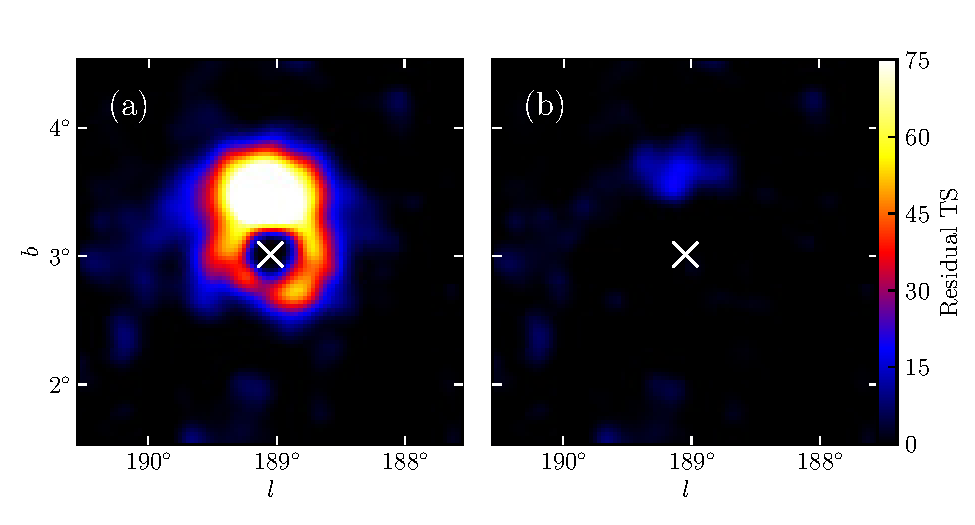
\includegraphics{chapters/extended_search/figures/ic443_plots/res_tsmap_ic443_color.pdf}
  \caption{A TS map generated for the region around the SNR IC~443 using
  photons with energies between 1 \gev and 100 \gev.  (a) TS map after
  subtracting IC~443 modeled as a point-like source. (b) same as (a),
  but IC~443 modeled as an extended source. The cross represents the
  best fit position of IC~443.}
  \figlabel{res_tsmaps}
\end{figure}

Similarly, many of these sources were confused with nearby point-like
sources or influenced by large-scale residuals in the diffuse emission.
To help determine which of these fits found truly extended sources
and when the extension was influenced by source confusion and diffuse
emission, we generated a series of diagnostic plots.  For each candidate,
we generated a map of the residual TS by adding a new point-like source
of spectral index 2 into the region at each position and finding the
increase in likelihood when fitting its flux. \figref{res_tsmaps} shows
this map around the most significantly extended source IC~443 when
it is modeled both as a point-like source and as an extended source.
The residual TS map indicates that the spatially extended model for
IC~443 is a significantly better description of the observed photons
and that there is no $\ts>25$ residual in the region after modeling the
source as being spatially extended.  We also generated plots of the
sum of all counts within a given distance of the source and compared
them to the model predictions assuming the emission originated from a
point-like source.  An example radial integral plot is shown for the
extended source IC~443 in \figref{four_plots_ic443}.  For each source,
we also made diffuse-emission-subtracted smoothed counts maps (shown
for IC~443 in \figref{four_plots_ic443}).

\begin{figure}[htbp]
    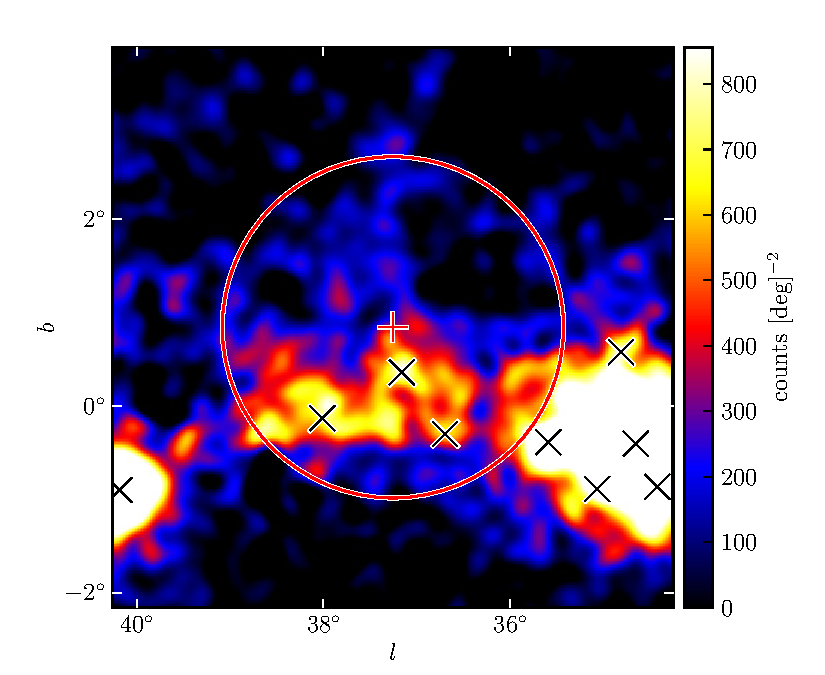
\includegraphics{source_plots/example_bad_fit_color.pdf}
    \caption{A diffuse-emission-subtracted 1 \gev to 100 \gev counts
    map of the region around 2FGL\,J1856.2+0450c smoothed by a 0\fdg1
    2D Gaussian kernel. The plus-shaped marker and circle (colored
    red in the online version) represent the center and size of the
    source fit with a radially-symmetric uniform disk spatial model.
    The black crosses represent the positions of other 2FGL sources.
    The extension is statistically significant, but the extension
    encompasses many 2FGL sources and the emission does not look to be
    uniform. Although the fit is statistically significant, it likely
    corresponds to residual features of inaccurately modeled diffuse
    emission picked up by the fit.}
    \figlabel{example_bad_fit}
\end{figure}

We found by visual inspection that in many cases our results were strongly
influenced by large-scale residuals in the diffuse emission and hence
the extension measure was unreliable.  This was especially true in our
analysis of sources in the 1 \gev to 100 \gev energy range.  An example
of such a case is 2FGL\,J1856.2+0450c analyzed in the 1 \gev to 100 \gev
energy range. \figref{example_bad_fit} shows a diffuse-emission-subtracted
smoothed counts map for this source with the best fit extension of
the source overlaid. There appear to be large-scale residuals in
the diffuse emission in this region along the Galactic plane.  As a
result, 2FGL\,J1856.2+0450c is fit to an extension of $\sim2\degree$
and the result is statistically significant with \tsext=45.4. However,
by looking at the residuals it is clear that this complicated region is
not well modeled. We manually discard sources like this.

We only selected extended source candidates in regions that did not
appear dominated by these issues and where there was a multiwavelength
counterpart. Because of these systematic issues, this search can not be
expected to be complete and it is likely that there are other spatially
extended sources that this method missed.


\begin{deluxetable}{lr}
\tablecolumns{2}
\tablewidth{0pt}
\tabletypesize{\small}
\tablecaption{Nearby Residual-induced Sources
\tablabel{fake_2fgl_sources}
}
\tablehead{
\colhead{Extended Source}&
\colhead{Residual-induced Sources}
}
\startdata
\hline
2FGL\,J0823.0$-$4246    & 2FGL\,J0821.0$-$4254, 2FGL\,J0823.4$-$4305 \\
2FGL\,J1627.0$-$2425c   & \nodata \\
2FGL\,J0851.7$-$4635    & 2FGL\,J0848.5$-$4535, 2FGL\,J0853.5$-$4711, 2FGL\,J0855.4$-$4625 \\
2FGL\,J1615.0$-$5051    & \nodata \\
2FGL\,J1615.2$-$5138    & 2FGL\,J1614.9$-$5212  \\
2FGL\,J1632.4$-$4753c   & 2FGL\,J1634.4$-$4743c \\
2FGL\,J1712.4$-$3941    & \nodata \\
2FGL\,J1837.3$-$0700c   & 2FGL\,J1835.5$-$0649 \\
2FGL\,J2021.5+4026      & 2FGL\,J2019.1+4040 \\
\enddata


\tablecomments{
For each new extended source, we list nearby 2FGL
soruces that we have concluded here correspond to residuals induced by not
modeling the extensions of nearby extended sources.
}
\end{deluxetable}



For each candidate that was not biased by neighboring point-like
sources or by large-scale residuals in the diffuse emission model, we
improved the model of the region by deciding on a case by case basis
which background point-like sources should be kept.  We kept in our
model the sources that we believed represented physically distinct
sources and we removed sources that we believed were included in the
2FGL catalog to compensate for residuals induced by not modeling the
extension of the source.  Soft nearby point-like 2FGL sources that
were not significant at higher energies were frozen to the spectras
predicted by 2FGL.  When deciding which background sources to keep and
which to remove, we used multiwavelength information about possibly
extended source counterparts to help guide our choice. For each extended
source presented in \secref{new_ext_srcs_section}, we describe any
modifications from 2FGL of the background model that were performed.
In \tabref{fake_2fgl_sources}, we summarize the sources in the 2FGL
catalog that we have concluded here correspond to residuals induced by
not modeling the extensions of nearby extended sources.

The best fit positions of nearby point-like sources can be influenced by
the extended source and vice versa.  Similarly, the best fit positions
of nearby point-like sources in the 2FGL catalog can be biased by
systematic issues at lower energies.  Therefore, after selecting the list
of background sources, we iteratively refit the positions and spectra
of nearby background sources as well as the positions and extensions of
the analyzed spatially extended sources until the overall fit converged
globally.  For each extended source, we will describe the positions of
any relocalized background sources.

After obtaining the overall best fit positions and extensions of all
of the sources in the region using \pointlike, we refit the spectral
parameters of the region using \gtlike.  With \gtlike, we obtained a
second measure of \tsext.  We only consider a source to be extended
when both \pointlike and \gtlike agree that $\tsext\ge16$.  We further
required that $\tsext\ge16$ using the alternative approach to modeling
the diffuse emission presented in \secref{systematic_errors_on_extension}.
We then replaced the spatially extended source with two point-like sources
and refit the positions and spectra of the two point-like sources to
calculate \tsinc.  We only consider a source to be spatially extended,
instead of being the result of confusion of two point-like sources,
if $\tsext>\tsinc$.  As was shown in \secref{dual_localization_method},
this test is fairly powerful at removing situations in which the emission
actually originates from two distinct point-like sources instead of one
spatially extended source.  On the other hand, it is still possible that
longer observations could resolve additional structure or new sources that
the analysis cannot currently detect.  Considering the very complicated
morphologies of extended sources observed at other wavelengths and
the high density of possible sources that are expected to emit at \gev
energies, it is likely that in some of these regions further observations
will reveal that the emission is significantly more complicated than
the simple radially-symmetric uniform disk model that we assume.

\section{New Extended Sources}
\seclabel{new_ext_srcs_section}


\thispagestyle{empty}
\begin{deluxetable}{lrrrrrrrrl}
\tablecolumns{10}
\tabletypesize{\small}
\rotate
\tablewidth{0pt}
\tablecaption{Extension fit for the nine additional extended sources
\tablabel{new_ext_srcs_table}
}
\tablehead{
\colhead{Name}&
\colhead{\glon}&
\colhead{\glat}&
\colhead{$\sigma$}&
\colhead{\ts}&
\colhead{\tsext}&
\colhead{Pos Err}&
\colhead{Flux\tablenotemark{(a)}}&
\colhead{Index}&
\colhead{Counterpart}\\
\colhead{}&
\colhead{(deg.)}&
\colhead{(deg.)}&
\colhead{(deg.)}&
\colhead{}&
\colhead{}&
\colhead{(deg.)}&
\colhead{}&
\colhead{}&
\colhead{}
}

\startdata
\multicolumn{10}{c}{E$>$1 \gev} \\
\hline
2FGL\,J0823.0$-$4246                       &     260.32 &    $-$3.28 & $  0.37 \pm   0.03 \pm   0.02 $ &      322.2 &       48.0 &   0.02 & $    8.4 \pm     0.6$ & $   2.21 \pm    0.09$ &                  Puppis A \\
2FGL\,J1627.0$-$2425c                      &     353.07 &      16.80 & $  0.42 \pm   0.05 \pm   0.16 $ &      139.9 &       32.4 &   0.04 & $    6.3 \pm     0.6$ & $   2.50 \pm    0.14$ &                 Ophiuchus \\
\cutinhead{E$>$10 \gev}
2FGL\,J0851.7$-$4635                       &     266.31 &    $-$1.43 & $  1.15 \pm   0.08 \pm   0.02 $ &      116.6 &       86.8 &   0.07 & $    1.3 \pm     0.2$ & $   1.74 \pm    0.21$ &                  Vela Jr. \\
2FGL\,J1615.0$-$5051                       &     332.37 &    $-$0.13 & $  0.32 \pm   0.04 \pm   0.01 $ &       50.4 &       16.7 &   0.04 & $    1.0 \pm     0.2$ & $   2.19 \pm    0.28$ &         HESS\,J1616$-$508 \\
2FGL\,J1615.2$-$5138                       &     331.66 &    $-$0.66 & $  0.42 \pm   0.04 \pm   0.02 $ &       76.1 &       46.5 &   0.04 & $    1.1 \pm     0.2$ & $   1.79 \pm    0.26$ &         HESS\,J1614$-$518 \\
2FGL\,J1632.4$-$4753c                      &     336.52 &       0.12 & $  0.35 \pm   0.04 \pm   0.02 $ &       64.4 &       26.9 &   0.04 & $    1.4 \pm     0.2$ & $   2.66 \pm    0.30$ &         HESS\,J1632$-$478 \\
2FGL\,J1712.4$-$3941\tablenotemark{(b)}    &     347.26 &    $-$0.53 & $  0.56 \pm   0.04 \pm   0.02 $ &       59.4 &       38.5 &   0.05 & $    1.2 \pm     0.2$ & $   1.87 \pm    0.22$ &        RX\,J1713.7$-$3946 \\
2FGL\,J1837.3$-$0700c                      &      25.08 &       0.13 & $  0.33 \pm   0.07 \pm   0.05 $ &       47.0 &       18.5 &   0.07 & $    1.0 \pm     0.2$ & $   1.65 \pm    0.29$ &         HESS\,J1837$-$069 \\
2FGL\,J2021.5+4026                         &      78.24 &       2.20 & $  0.63 \pm   0.05 \pm   0.04 $ &      237.2 &      128.9 &   0.05 & $    2.0 \pm     0.2$ & $   2.42 \pm    0.19$ &            $\gamma$-Cygni \\
\enddata

\tablenotetext{(a)}{
Integral Flux in units of $10^{-9}$ \fluxunits and integrated in the fit
energy range (either 1 \gev to 100 \gev or 10 \gev to 100 \gev).
}

\tablenotetext{(b)}{
The discrepancy in the best fit spectra of 2FGL\,J1712.4$-$3941 compared
to \cite{abdo_2011a_observations-young} is due to fitting over a different energy range.
}


\tablecomments{
    The columns in this table have the same meaning as those in
    \tabref{known_extended_sources}.
    RX\,J1713.7$-$3946 and Vela Jr. were previously studied in dedicated publications \citep{abdo_2011a_observations-young,tanaka_2011a_gamma-ray-observations}.
}
\end{deluxetable}




\thispagestyle{empty}
\begin{deluxetable}{lrrrrrrrrrr}
  \tabletypesize{\scriptsize}
  \tablecolumns{11}
  \rotate
  \tablewidth{0pt}
  \tablecaption{Dual localization, alternative PSF, and alternative approach to modeling the diffuse emission
  \tablabel{alt_diff_model_results}
  }
  \tablehead{
  \colhead{Name}&
  \colhead{$\tspointlike$}&
  \colhead{$\tsgtlike$}&
  \colhead{$\tsaltdiff$}&
  \colhead{$\tsextpointlike$}&
  \colhead{$\tsextgtlike$}&
  \colhead{$\tsextaltdiff$}&
  \colhead{$\sigma$}&
  \colhead{$\sigma_\altdiff$}&
  \colhead{$\sigma_\altpsf$}&
  \colhead{$\tsinc$}\\
  \colhead{}&
  \colhead{}&
  \colhead{}&
  \colhead{}&
  \colhead{}&
  \colhead{}&
  \colhead{}&
  \colhead{(deg.)}&
  \colhead{(deg.)}&
  \colhead{(deg.)}&
  \colhead{}
  }
  \startdata
\multicolumn{11}{c}{E$>$1 \gev} \\[3pt]
\hline
2FGL\,J0823.0$-$4246      &                331.9 &                322.2 &                356.0 &                 60.0 &                 48.0 &                 56.0 &                 0.37 &                 0.39 &                 0.39 &                 23.0 \\
2FGL\,J1627.0$-$2425c     &                154.8 &                139.9 &                105.7 &                 39.4 &                 32.4 &                 24.8 &                 0.42 &                
 0.40 &                 0.58 &                 24.5 \\
\hline\\[-4pt]
\multicolumn{11}{c}{E$>$10 \gev} \\[3pt]
\hline
2FGL\,J0851.7$-$4635      &                115.2 &                116.6 &                123.1 &                 83.9 &                 86.8 &                 89.8 &                 1.15 &                 1.16 &                 1.17 &                 15.5 \\
2FGL\,J1615.0$-$5051\tablenotemark{(a)} &                 48.2 &                 50.4 &                 56.6 &                 15.2 &                 16.7 &                 17.8 &                 0.32 &                 0.33 &                 0.32 &                 13.1 \\
2FGL\,J1615.2$-$5138      &                 75.0 &                 76.1 &                 83.8 &                 42.9 &                 46.5 &                 54.1 &                 0.42 &                 0.43 &                 0.43 &                 35.1 \\
2FGL\,J1632.4$-$4753c     &                 64.5 &                 64.4 &                 66.8 &                 23.0 &                 26.9 &                 25.5 &                 0.35 &                 0.36 &                 0.37 &                 10.9 \\
2FGL\,J1712.4$-$3941      &                 59.8 &                 59.4 &                 39.9 &                 38.4 &                 38.5 &                 30.7 &                 0.56 &                 0.55 &                 0.53 &                  2.7 \\
2FGL\,J1837.3$-$0700c     &                 44.5 &                 47.0 &                 39.2 &                 17.6 &                 18.5 &                 16.1 &                 0.33 &                 0.32 &                 0.38 &                 10.8 \\
2FGL\,J2021.5+4026        &                239.1 &                237.2 &                255.8 &                139.1 &                128.9 &                138.0 &                 0.63 &                 0.65 &                 0.59 &                 37.3 \\
  \enddata

\tablenotetext{(a)}{
Using \pointlike, \tsext for 2FGL\,J1615.0$-$5051 was sligthly below
16 when the source was fit in the 10 \gev to 100 \gev energy range. To
confirm the extension measure, the extension was refit in \pointlike
using a slightly lower energy.  In the 5.6 \gev to 100 \gev energy range,
we obtained a consistent extension and \tsext=28.0.  In the rest of
this paper, we quote the $E>10 \gev$ results for consistency with the
other sources.
}

\tablecomments{
$\tspointlike$, $\tsgtlike$, and $\tsaltdiff$ are the test
statistic values from \pointlike, \gtlike, and \gtlike with the alternative
approach to modeling the diffuse emission respectively.  $\tsextpointlike$, $\tsextgtlike$,
and $\tsextaltdiff$ are the TS values from \pointlike, \gtlike, and \gtlike with the alternative 
approach to modeling the diffuse emission respectively.  $\sigma$, $\sigma_\altdiff$, and $\sigma_\altpsf$
are the fit sizes assuming
a radially-symmetric uniform disk model
with the standard analysis, the alternative 
approach to modeling the diffuse emission, and the alternative PSF respectively.  
}
\end{deluxetable}


Nine extended sources not included in the 2FGL catalog were found
by our extended source search. Two of these have been previously
studied in dedicated publications: RX\,J1713.7$-$3946 and Vela Jr.
\citep{abdo_2011a_observations-young,tanaka_2011a_gamma-ray-observations}.
Two of these sources were found when using photons with energies
between 1 \gev and 100 \gev and seven were found when using photons
with energies between 10 \gev and 100 \gev.  For the sources found at
energies above 10 \gev, we restrict our analysis to higher energies
because of the issues of source confusion and diffuse emission modeling
described in \secref{extended_source_search_method}.  The spectral
and spatial properties of these nine sources are summarized in
\tabref{new_ext_srcs_table} and the results of our investigation of
systematic errors are presented in \tabref{alt_diff_model_results}.
\tabref{alt_diff_model_results} also compares the likelihood assuming
the source is spatially extended to the likelihood assuming that the
emission originates from two independent point-like sources. For
these new extended sources, $\tsext>\tsinc$ so we conclude that
the \gev emission does not originate from two physically distinct
point-like sources (see \secref{dual_localization_method}).
\tabref{alt_diff_model_results} also includes the results of the
extension fits using variations of the PSF and the Galactic diffuse model
described in \secref{systematic_errors_on_extension}.  There is good
agreement between \tsext and the fit size using the standard analysis,
the alternative approach to modeling the diffuse emission, and the
alternative PSF.  This suggests that the sources are robust against
mis-modeled features in the diffuse emission model and uncertainties in
the PSF.

\subsection{2FGL\,J0823.0$-$4246}
\subseclabel{section_2FGL_J0823.0-4246}

\begin{figure}[htbp]
  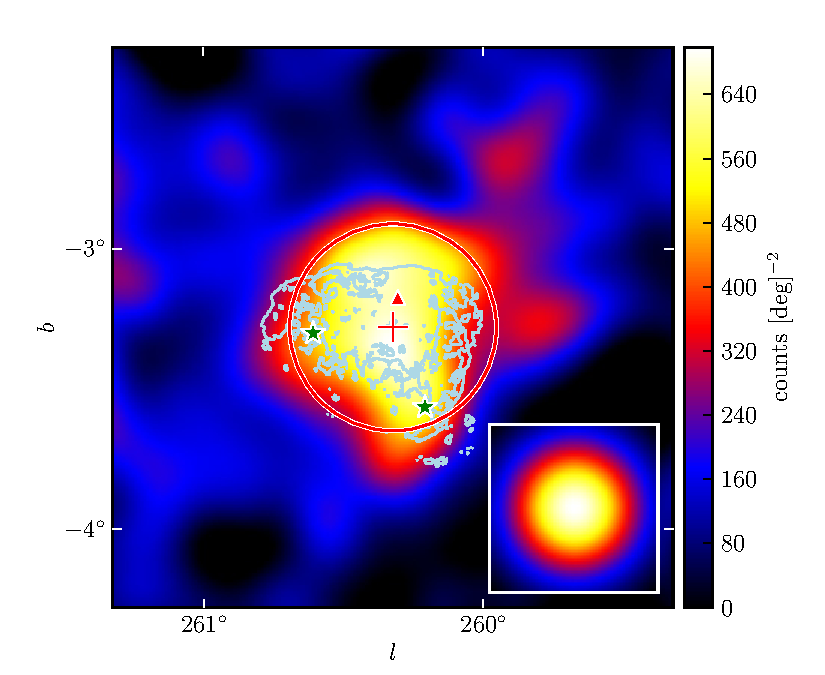
\includegraphics{source_plots/source_Puppis_A_color.pdf}
  \caption{A diffuse-emission-subtracted 1 \gev to 100 \gev counts
  map of 2FGL\,J0823.0$-$4246 smoothed by a 0\fdg1 2D Gaussian kernel.
  The triangular marker (colored red in the online version) represents the
  2FGL position of this source.  The plus-shaped marker and the circle
  (colored red) represent the best fit position and extension of this
  source assuming a radially-symmetric uniform disk model.  The two
  star-shaped markers (colored green) represent 2FGL sources that were
  removed from the background model.  From left to right, these sources
  are 2FGL\,J0823.4$-$4305 and 2FGL\,J0821.0$-$4254.  The lower right
  inset is the model predicted emission from a point-like source with
  the same spectrum as 2FGL\,J0823.4$-$4305 smoothed by the same kernel.
  This source is spatially coincident with the Puppis A SNR. The light
  blue contours correspond to the X-ray image of Puppis A observed by
  \rosat \citep{petre_1996a_central-stellar}.}
  \figlabel{1FGL_J0823.3-4248}
\end{figure}

2FGL\,J0823.0$-$4246 was found by our search to be an extended source
candidate in the 1 \gev to 100 \gev energy range and is spatially
coincident with the SNR Puppis A.  \figref{1FGL_J0823.3-4248}
shows a counts map of this source. There are two nearby 2FGL sources
2FGL\,J0823.4$-$4305 and 2FGL\,J0821.0$-$4254 that are also coincident
with the SNR but that do not appear to represent physically distinct
sources.  We conclude that these nearby point-like sources were included
in the 2FGL catalog to compensate for residuals induced by not modeling
the extension of this source and removed them from our model of the sky.
After removing these sources, 2FGL\,J0823.0$-$4246 was found to have
an extension $\sigma=0\fdg37\pm0\fdg03_\stat\pm0\fdg02_\sys$ with
$\tsext=48.0$.  \figref{snr_seds} shows the spectrum of this source.

Puppis A has been studied in detail in radio
\citep{castelletti_2006a_observations-puppis}, and  X-ray
\citep{petre_1996a_central-stellar,hwang_2008a_x-ray-emitting-ejecta}.
The fit extension of 2FGL\,J0823.0$-$4246 matches well the size of
Puppis A in X-ray.  The distance of Puppis A was estimated at 2.2 kpc
\citep{reynoso_1995a_observations-neutral,reynoso_2003a_observations-neutral}
and leads to a 1 \gev to 100 \gev luminosity of $\sim 3\times 10^{34}$
ergs$\,\second^{-1}$.  No molecular clouds have been observed directly
adjacent to Puppis A \citep{paron_2008a_high-resolution-observations},
similar to the LAT-detected Cygnus Loop SNR
\citep{katagiri_2011a_fermi-large}.  The luminosity of Puppis A is also
smaller than that of other SNRs believed to interact with molecular clouds
\citep{abdo_2009a_fermi-discovery,abdo_2010a_observation-supernova,abdo_2010a_gamma-ray-emission,abdo_2010d_fermi-large,abdo_2010a_fermi-lat-study}.

\subsection{2FGL\,J0851.7$-$4635}
\subseclabel{section_2FGL_J0851.7-4635}

\begin{figure}[htbp]
  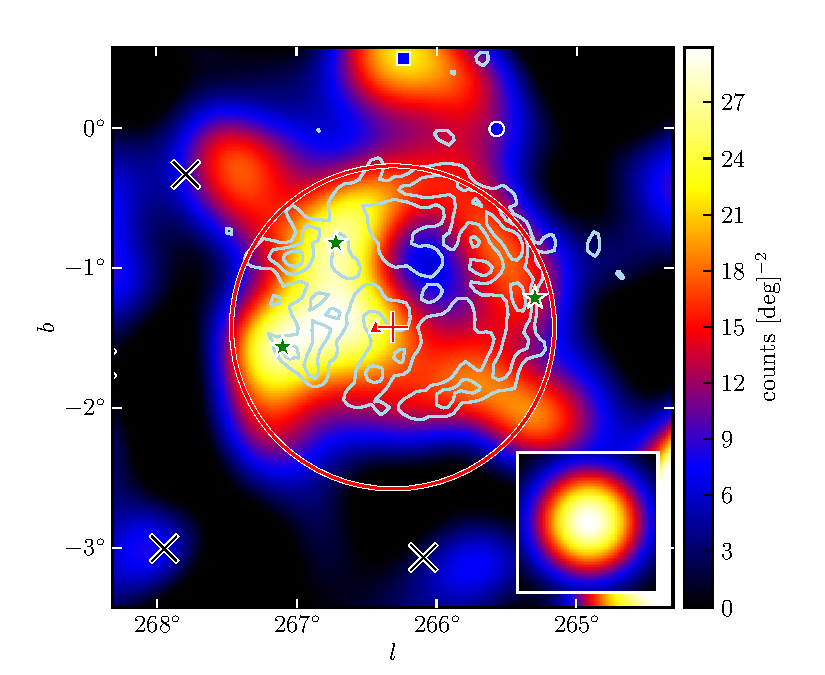
\includegraphics{source_plots/source_Vela_Jr_color.pdf}
  \caption{A diffuse-emission-subtracted 10 \gev to 100 \gev counts map
  of 2FGL\,J0851.7$-$4635 smoothed by a 0\fdg25 2D Gaussian kernel. The
  triangular marker (colored red in the electronic version) represents the
  2FGL position of this source.  The plus-shaped marker and the circle
  (colored red) are the best fit position and extension of this source
  assuming a radially-symmetric uniform disk model.  The three black
  crosses represent background 2FGL sources.  The three star-shaped
  markers (colored green) represent other 2FGL sources that were
  removed from the background model.  They are (from left to right)
  2FGL\,J0853.5$-$4711, 2FGL\,J0855.4$-$4625, and 2FGL\,J0848.5$-$4535.
  The circular and square-shaped marker (colored blue) represents the
  2FGL and relocalized position of another 2FGL source.  This extended
  source is spatially coincident with the Vela Jr. SNR.  The contours
  (colored light blue) correspond to the \tev image of Vela Jr.
  \citep{aharonian_2007a_h.e.s.s.-observations}.}
  \figlabel{Vela_Jr}
\end{figure}

2FGL\,J0851.7$-$4635 was found by our search to be an extended source
candidate in the 10 \gev to 100 \gev energy range and is spatially
coincident with the SNR Vela Jr. This source was recently studied by
the LAT Collaboration in \cite{tanaka_2011a_gamma-ray-observations}.
\figref{Vela_Jr} shows a counts map of the source.
Overlaid on \figref{Vela_Jr} are \tev contours of Vela
Jr. \citep{aharonian_2007a_h.e.s.s.-observations}.  There are three
point-like 2FGL sources 2FGL\,J0848.5$-$4535, 2FGL\,J0853.5$-$4711, and
2FGL\,J0855.4$-$4625 which correlate with the multiwavelength emission of
this SNR but do not appear to be physically distinct sources.  They were
most likely included in the 2FGL catalog to compensate for residuals
induced by not modeling the extension of Vela Jr. and were removed from
our model of the sky.

With this model of the background, 2FGL\,J0851.7$-$4635 was found to
have an extension of $\sigma=1\fdg15\pm0\fdg08_\stat\pm0\fdg02_\sys$
with $\tsext=86.8$.  The LAT size matches well the \tev morphology
of Vela Jr.  While fitting the extension of 2FGL\,J0851.7$-$4635,
we iteratively relocalized the position of the nearby point-like 2FGL
source 2FGL\,J0854.7$-$4501 to $(l,b)=(266\fdg24,0\fdg49)$ to better
fit its position at high energies.
    
\subsection{2FGL\,J1615.0$-$5051}
\subseclabel{section_2FGL_J1615.0-5051}

\begin{figure}[htbp]
  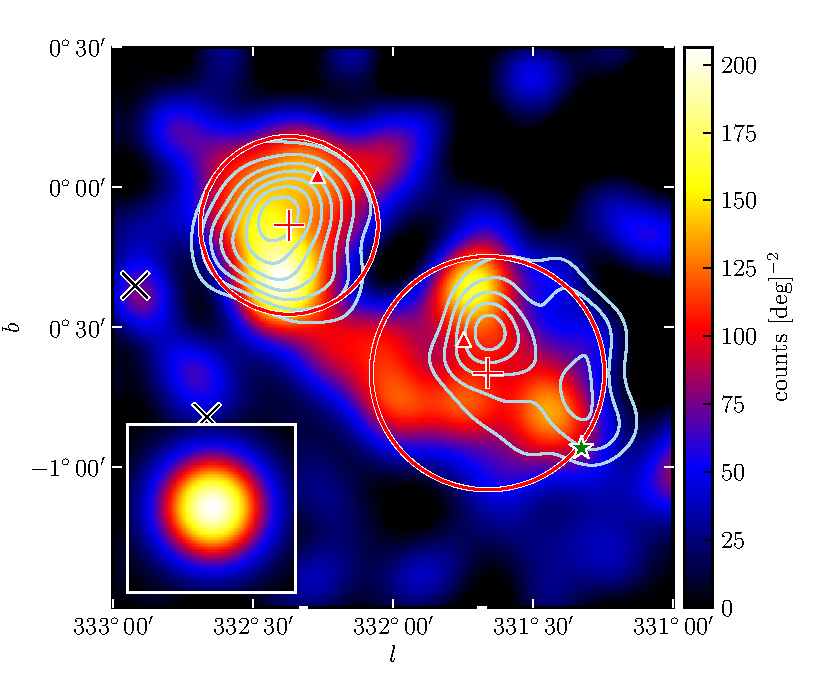
\includegraphics{source_plots/source_HESS_J1614-518_color.pdf}
  \caption{A diffuse-emission-subtracted 10 \gev to 100 \gev counts map
  of 2FGL\,J1615.0$-$5051 (upper left) and 2FGL\,J1615.2$-$5138 (lower
  right) smoothed by a 0\fdg1 2D Gaussian kernel.  The triangular markers
  (colored red in the electronic version) represent the 2FGL positions
  of these sources.  The cross-shaped markers and the circles (colored
  red) represent the best fit positions and extensions of these sources
  assuming a radially symmetric uniform disk model.  The two black
  crosses represent  background 2FGL sources and the star-shaped marker
  (colored green) represents 2FGL J1614.9-5212, another 2FGL source
  that was removed from the background model. The contours (colored
  light blue) correspond to the \tev image of HESS\,J1616$-$508 (left)
  and HESS\,J1614$-$518 (right) \citep{aharonian_2006a_h.e.s.s.-survey}.}
  \figlabel{1FGL_J1613.6-5100c}
\end{figure}

2FGL\,J1615.0$-$5051 and 2FGL\,J1615.2$-$5138 were both found to
be extended source candidates in the 10 \gev to 100 \gev energy
range. Because they are less than $1\degree$ away from each other,
they needed to be analyzed simultaneously.  2FGL\,J1615.0$-$5051 is
spatially coincident with the extended \tev source HESS\,J1616$-$508
and 2FGL\,J1615.2$-$5138 is coincident with the extended \tev source
HESS\,J1614$-$518.  \figref{1FGL_J1613.6-5100c} shows a counts map of
these sources and overlays the \tev contours of HESS\,J1616$-$508 and
HESS\,J1614$-$518 \citep{aharonian_2006a_h.e.s.s.-survey}.  The figure
shows that the 2FGL source 2FGL\,J1614.9$-$5212 is very close to
2FGL\,J1615.2$-$5138 and correlates with the same extended \tev source
as 2FGL\,J1615.2$-$5138.  We concluded that this source was included
in the 2FGL catalog to compensate for residuals induced by not modeling
the extension of 2FGL\,J1615.2$-$5138 and removed it from our model of
the sky.

With this model of the sky, we iteratively fit the extensions of
2FGL\,J1615.0$-$5051 and 2FGL\,J1615.2$-$5138.  2FGL\,J1615.0$-$5051 was
found to have an extension $\sigma=0\fdg32\pm0\fdg04_\stat\pm0\fdg01_\sys$
and \tsext=16.7.

The \tev counterpart of 2FGL\,J1615.0$-$5051 was fit with
a radially-symmetric Gaussian surface brightness profile with
$\sigma=0\fdg136\pm0\fdg008$ \citep{aharonian_2006a_h.e.s.s.-survey}. This
\tev size corresponds to a 68\% containment radius of
$\rsixeight=0\fdg21\pm0\fdg01$, comparable to the LAT size
$\rsixeight=0\fdg26\pm0\fdg03$.  \figref{hess_seds} shows that the
spectrum of 2FGL\,J1615.0$-$5051 at \gev energies connects to the spectrum
of HESS\,J1616$-$508 at \tev energies.

HESS\,J1616$-$508 is located in the region of two SNRs RCW103 (G332.4-04)
and Kes~32 (G332.4+0.1) but is not spatially coincident with either of
them \citep{aharonian_2006a_h.e.s.s.-survey}.  HESS\,J1616$-$508 is near
three pulsars PSR\,J1614$-$5048, PSR\,J1616$-$5109, and PSR\,J1617$-$5055.
\citep{torii_1998a_discovery-millisecond,landi_2007a_j1616-508:-likely}.
Only PSR\,J1617$-$5055 is energetically capable of powering the
\tev emission and \cite{aharonian_2006a_h.e.s.s.-survey} speculated
that HESS\,J1616$-$508 could be a PWN powered by this young pulsar.
Because HESS\,J1616$-$508 is $9\arcmin$ away from PSR\,J1617$-$5055,
this would require an asymmetric X-ray PWNe to power the \tev
emission.  \chandra ACIS observations revealed an underluminous
PWN of size $\sim1\arcmin$ around the pulsar that was not oriented
towards the \tev emission, rendering this association uncertain
\citep{kargaltsev_2008a_young-energetic}.  No other promising counterparts
were observed at X-ray and soft $\gamma$-ray energies by \suzaku
\citep{matsumoto_2007a_suzaku-observations}, \swiftxrt, IBIS/ISGRBI,
BeppoSAX and \xmmnewton \citep{landi_2007a_j1616-508:-likely}.
\cite{kargaltsev_2008a_young-energetic} discovered additional diffuse
emission towards the center of HESS\,J1616$-$508 using archival radio
and infared observations. Deeper observations will likely be necessary
to understand this $\gamma$-ray source.

\subsection{2FGL\,J1615.2$-$5138}
\subseclabel{section_2FGL_J1615.2-5138}

2FGL\,J1615.2$-$5138 was found
 to have an extension $\sigma=0\fdg42\pm0\fdg04_\stat\pm0.02_\sys$
with $\tsext=46.5$.  To test for the possibility that 2FGL\,J1615.2$-$5138
is not spatially extended but instead composed of two point-like sources
(one of them represented in the 2FGL catalog by 2FGL\,J1614.9$-$5212),
we refit 2FGL\,J1615.2$-$5138 as two point-like sources.  Because
$\tsinc=35.1$ is less than $\tsext=46.5$, we conclude that this emission
does not originate from two closely-spaced point-like sources.

2FGL\,J1615.2$-$5138 is spatially coincident with the extended \tev
source HESS\,J1614$-$518.  \ac{HESS} measured a 2D Gaussian extension
of $\sigma=0\fdg23\pm0\fdg02$ and $\sigma=0\fdg15\pm0\fdg02$ in the
semi-major and semi-minor axis. This corresponds to a 68\% containment
size of $\rsixeight=0\fdg35\pm0\fdg03$ and $0\fdg23\pm0\fdg03$,
consistent with the LAT size $\rsixeight=0\fdg34\pm0\fdg03$.
\figref{hess_seds} shows that the spectrum of 2FGL\,J1615.2$-$5138
at \gev energies connects to the spectrum of HESS\,J1614$-$518 at
\tev energies.  Further data collected by \ac{HESS} in 2007 resolve
a double peaked structure at \tev energies but no spectral variation
across this source, suggesting that the emission is not the confusion of
physically separate sources \citep{rowell_2008a_closer-unidentified}.
This double peaked structure is also hinted at in the LAT
counts map in \figref{1FGL_J1613.6-5100c} but is not very
significant.  The \tev source was also detected by CANGAROO-III
\citep{mizukami_2011a_cangaroo-iii-observation}.

There are five nearby pulsars, but none are luminous enough to provide
the energy output required to power the $\gamma$-ray emission
\citep{rowell_2008a_closer-unidentified}.  HESS\,J1614$-$518
is spatially coincident with a young open cluster Pismis 22
\citep{landi_2007a_j1614-518:-detection,rowell_2008a_closer-unidentified}.
\suzaku detected two promising X-ray candidates. Source A is an extended
source consistent with the peak of HESS\,J1614$-$518 and source B
coincident with Pismis 22 and towards the center but in a relatively dim
region of HESS\,J1614$-$518 \citep{matsumoto_2008a_discovery-extended}.
Three hypotheses have been presented to explain this emission: either
source A is an SNR powering the $\gamma$-ray emission; source A is a PWN
powered by an undiscovered pulsar in either source A or B; and finally
that the emission may arise from hadronic acceleration in the stellar
winds of Pismis 22 \citep{mizukami_2011a_cangaroo-iii-observation}.

\subsection{2FGL\,J1627.0$-$2425c}
\subseclabel{section_2FGL_J1627.0-2425c}

\begin{figure}[htbp]
  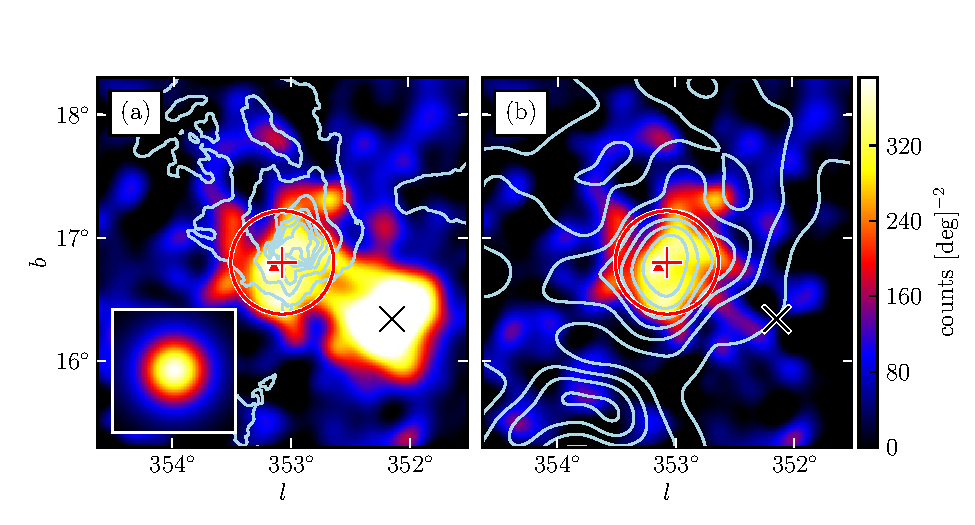
\includegraphics{source_plots/source_Ophiuchus_color.pdf}
  \caption{A diffuse-emission-subtracted 1 \gev to 100 \gev counts map
  of (a) the region around 2FGL\,J1627.0$-$2425 smoothed by a 0\fdg1 2D
  Gaussian kernel and (b) with the emission from 2FGL\,J1625.7$-$2526
  subtracted.  The triangular marker (colored red in the online version)
  represents the 2FGL position of this source.  The plus-shaped
  marker and the circle (colored red) represent the best fit position
  and extension of this source assuming a radially-symmetric uniform
  disk model and the black cross represents a background 2FGL source.
  The contours in (a) correspond to the 100 $\mu$m image observed by
  IRAS \citep{young_1986a_high-resolution-observations}.  The contours
  in (b) correspond to CO ($J=1\rightarrow 0$) emission integrated
  from $-$8 $\km\,\second^{-1}$ to 20 $\km\,\second^{-1}$.  They are
  from \cite{de-geus_1990a_survey-clouds}, were cleaned using the
  moment-masking technique \citep{dame_2011a_optimization-moment},
  and have been smoothed by a 0\fdg25 2D Gaussian kernel.}
  \figlabel{1FGL_J1628.6-2419c}
\end{figure}

2FGL\,J1627.0$-$2425c was found by our search to have an extension
$\sigma=0\fdg42\pm0\fdg05_\stat\pm0\fdg16_\sys$ with $\tsext=32.4$
using photons with energies between 1 \gev and 100 \gev.
\figref{1FGL_J1628.6-2419c} shows a counts map of this source.

This source is in a region of remarkably complicated diffuse emission.
Even though it is $16\degree$ from the Galactic plane, this source
is on top of the core of the Ophiuchus molecular cloud which
contains massive star-forming regions that are bright in infrared.
The region also has abundant molecular and atomic gas traced by CO
and H~I and significant dark gas found only by its association with
dust emission \citep{grenier_2005a_unveiling-extensive}. Embedded
star-forming regions make it even more challenging to measure
the column density of dust.  Infared and CO ($J=1\rightarrow
0$) contours are overlaid on \figref{1FGL_J1628.6-2419c}
and show good spatial correlation with the \gev emission
\citep{young_1986a_high-resolution-observations,de-geus_1990a_survey-clouds}.
This source might represent $\gamma$-ray emission from the interactions
of cosmic rays with interstellar gas which has not been accounted for
in the LAT diffuse emission model.

\subsection{2FGL\,J1632.4$-$4753c}
\subseclabel{section_2FGL_J1632.4-4753c}

\begin{figure}[htbp]
  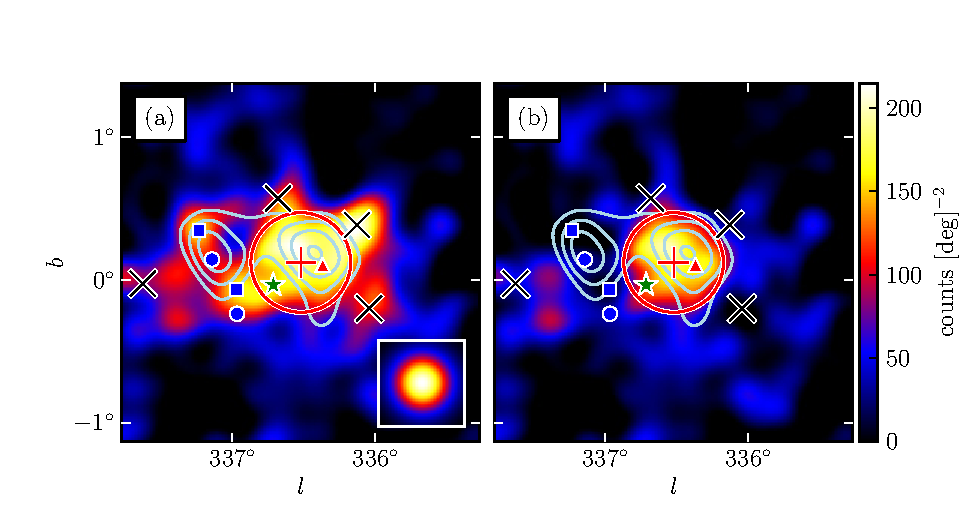
\includegraphics{source_plots/source_HESS_J1632-478_color.pdf}
  \caption{A diffuse-emission-subtracted 10 \gev to 100 \gev counts map
  of 2FGL\,J1632.4$-$4753c (a) smoothed by a 0\fdg1 2D Gaussian kernel
  and (b) with the emission from the background sources subtracted.
  The triangular marker (colored red in the electronic version)
  represents the 2FGL position of this source.  The plus-shaped marker
  and the circle (colored red) are the best fit position and extension of
  2FGL\,J1632.4$-$4753c assuming a radially-symmetric uniform disk model.
  The four black crosses represent background 2FGL sources subtracted in
  (b).  The circular and square-shaped markers (colored blue) represent
  the 2FGL and relocalized positions respectively of two additional
  background 2FGL sources subtracted in (b).  The star-shaped marker
  (colored green) represents 2FGL\,J1634.4$-$4743c, another 2FGL
  source that was removed from the background model.  The contours
  (colored light blue) correspond to the \tev image of HESS\,J1632$-$478
  \citep{aharonian_2006a_h.e.s.s.-survey}.}
  \figlabel{1FGL_J1632.9-4802c}
\end{figure}

2FGL\,J1632.4$-$4753c was found by our search to be an extended
source candidate in the 10 \gev to 100 \gev energy range but is in a
crowded region of the sky.  It is spatially coincident with the \tev
source HESS\,J1632$-$478.  \figref{1FGL_J1632.9-4802c}a shows a counts
map of this source and overlays \tev contours of HESS\,J1632$-$478
\citep{aharonian_2006a_h.e.s.s.-survey}.  There are six nearby
point-like 2FGL sources that appear to represent physically distinct
sources and were included in our background model: 2FGL\,J1630.2$-$4752,
2FGL\,J1631.7$-$4720c, 2FGL\,J1632.4$-$4820c, 2FGL\,J1635.4$-$4717c,
2FGL\,J1636.3$-$4740c, and 2FGL\,J1638.0$-$4703c. On the other hand,
one point-like 2FGL source 2FGL\,J1634.4$-$4743c  correlates with the
extended \tev source and at \gev energies does not appear physically
separate.  It is very close to the position of 2FGL\,J1632.4$-$4753c
and does not show spatially separated emission in the observed
photon distribution.  We therefore removed this source from our
model of the background.  \figref{1FGL_J1632.9-4802c}b shows the
same region with the background sources subtracted.  With this
model, 2FGL\,J1632.4$-$4753c was found to have an extension
$\sigma=0\fdg35\pm0\fdg04_\stat\pm0\fdg02_\sys$ with $\tsext=26.9$.
While fitting the extension of 2FGL\,J1632.4$-$4753c, we iteratively
relocalized 2FGL\,J1635.4$-$4717c to $(l,b)=(337\fdg23,0\fdg35)$ and
2FGL\,J1636.3$-$4740c to $(l,b)=(336\fdg97,-0\fdg07)$.

\begin{figure}[htbp]
  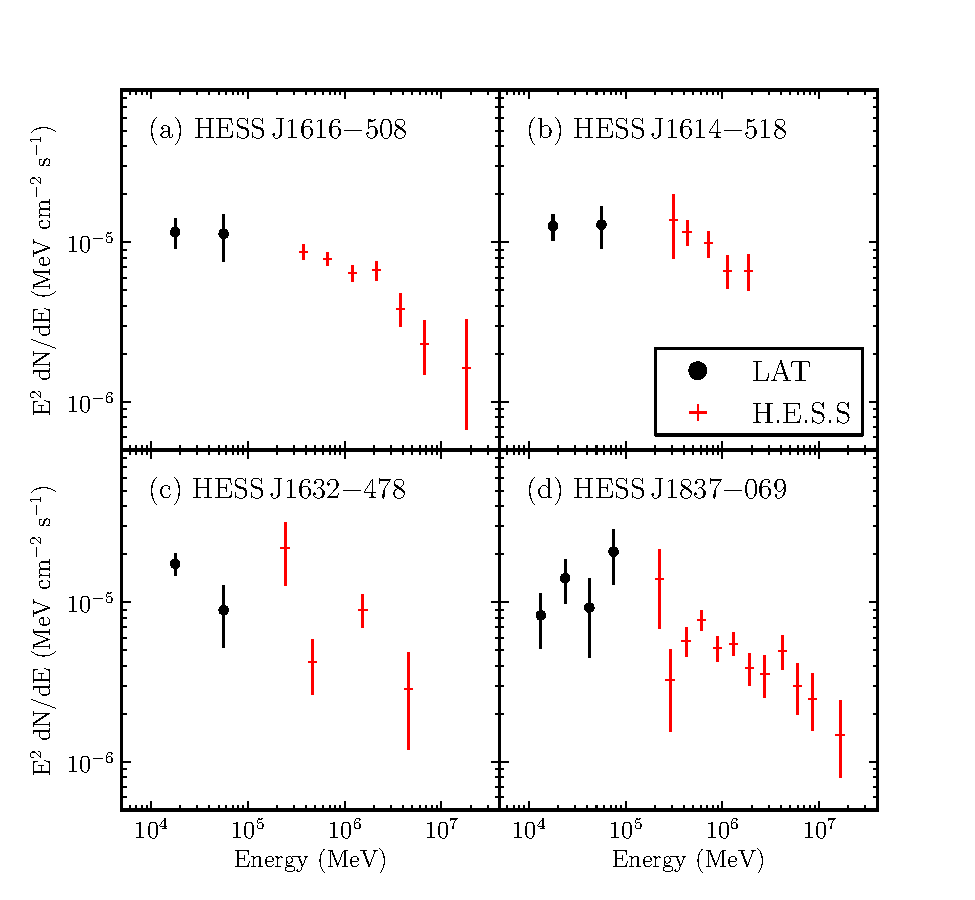
\includegraphics{chapters/extended_search/figures/summary_plots/hess_seds_color.pdf}
  \caption{The spectral energy distribution of four extended
  sources associated with unidentified extended \tev sources.
  The black points with circular markers are obtained by the
  LAT. The points with plus-shaped markers (colored red in the
  electronic version) are for the associated \ac{HESS} sources.
  (a) the LAT SED of 2FGL\,J1615.0$-$5051 together with the
  \ac{HESS} SED of HESS\,J1616$-$508. (b) 2FGL\,J1615.2$-$5138 and
  HESS\,J1614$-$518. (c) 2FGL\,J1632.4$-$4753c and HESS\,J1632$-$478. (d)
  2FGL\,J1837.3$-$0700c and HESS\,J1837$-$069. The \ac{HESS} data points
  are from \citep{aharonian_2006a_h.e.s.s.-survey}. Both LAT and \ac{HESS}
  spectral errors are statistical only.}
    \figlabel{hess_seds}
  \end{figure}

\ac{HESS} measured an extension of $\sigma=0\fdg21\pm0\fdg05$ and
$0\fdg06\pm0\fdg04$ along the semi-major and semi-minor axes when
fitting HESS\,J1632$-$478 with an elliptical 2D Gaussian surface
brightness profile.  This corresponds to a 68\% containment size
$\rsixeight=0\fdg31\pm0\fdg08$ and $0\fdg09\pm0\fdg06$ along
the semi-major and semi-minor axis, consistent with the LAT size
$\rsixeight=0\fdg29\pm0\fdg04$.  \figref{hess_seds} shows that the
spectrum of 2FGL\,J1632.4$-$4753c at \gev energies connects to the
spectrum of HESS\,J1632$-$478 at \tev energies.

\cite{aharonian_2006a_h.e.s.s.-survey} argued that
HESS\,J1632$-$478 is positionally coincident with the hard X-ray
source IGR\,J1632$-$4751 observed by \asca, INTEGRAL, and \xmmnewton
\citep{sugizaki_2001a_faint-x-ray,tomsick_2003a_j16320-4751,rodriguez_2003a_xmm-newton-observation},
but this source is suspected to be a Galactic X-Ray Binary so the
$\gamma$-ray extension disfavors the association.  Further observations
by \xmmnewton discovered point-like emission coincident with the
peak of the \ac{HESS} source surrounded by extended emission of size
$\sim32\arcsec\times15\arcsec$ \citep{balbo_2010a_j1632-478:-energetic}.
They found in archival MGPS-2 data a spatially coincident extended
radio source \citep{murphy_2007a_second-epoch} and argued for a
single synchrotron and inverse Compton process producing the radio,
X-ray, and \tev emission, likely due to a PWN.  The increased
size at \tev energies compared to X-ray energies has previously
been observed in several aging PWNe including HESS\,J1825$-$137
\citep{gaensler_2003a_xmm-newton-observations,aharonian_2006a_energy-dependent},
HESS\,J1640$-$465
\citep{aharonian_2006a_h.e.s.s.-survey,funk_2007a_xmm-newton-observations},
and Vela X
\citep{markwardt_1995a_x-ray-pulsar,aharonian_2006a_first-detection}
and can be explained by different synchrotron cooling times for the
electrons that produce X-rays and $\gamma$-rays.

\subsection{2FGL\,J1712.4$-$3941}
\subseclabel{section_2FGL_J1712.4-3941}

\begin{figure}[htbp]
  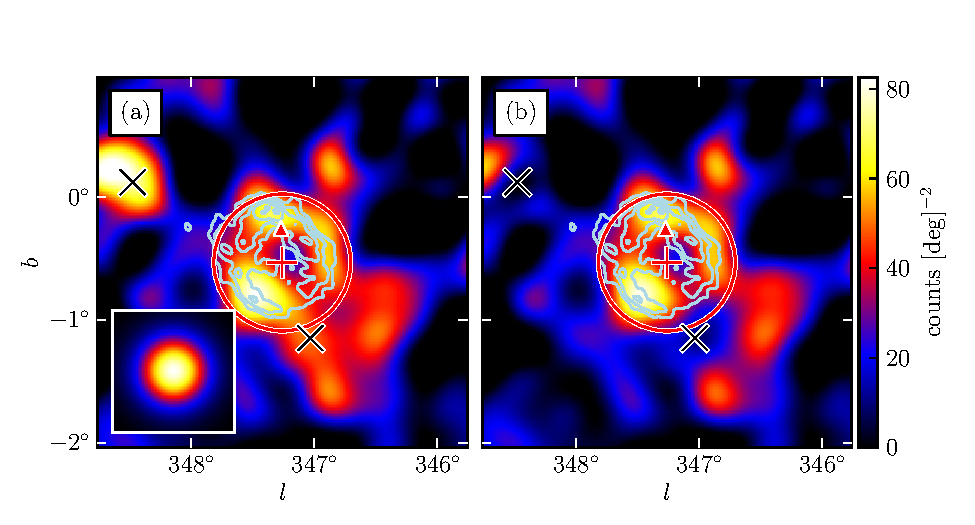
\includegraphics{source_plots/source_RX_J1713d7-3946_color.pdf}
  \caption{A diffuse-emission-subtracted 10 \gev to 100 \gev counts map
  of 2FGL\,J1712.4$-$3941 (a) smoothed by a 0\fdg15 2D Gaussian kernel
  and (b) with the emission from the background sources subtracted.
  This source is spatially coincident with RX\,J1713.7$-$3946 and
  was recently studied in \cite{abdo_2011a_observations-young}.
  The triangular marker (colored red in the online version) represents
  the 2FGL position of this source.  The plus-shaped marker and the
  circle (colored red) are the best fit position and extension of this
  source assuming a radially symmetric uniform disk model.  The two
  black crosses represent background 2FGL sources subtracted in (b).
  The contours (colored light blue) correspond to the \tev image
  \citep{aharonian_2007a_primary-particle}.}
  \figlabel{2FGL_J1712.4-3941}
\end{figure}

2FGL\,J1712.4$-$3941 was found by our search to be spatially extended
using photons with energies between 1 \gev and 100 \gev.  This source
is spatially coincident with the SNR RX\,J1713.7$-$3946 and was recently
studied by the LAT Collaboration in \cite{abdo_2011a_observations-young}.
To avoid issues related to uncertainties in the nearby Galactic
diffuse emission at lower energy, we restricted our analysis only
to energies above 10 \gev.  \figref{2FGL_J1712.4-3941} shows a
smoothed counts map of the source. Above 10 \gev, the \gev emission
nicely correlates with the \tev contours of RX\,J1713.7$-$3946
\citep{aharonian_2007a_primary-particle} and 2FGL\,J1712.4$-$3941 fit
to an extension $\sigma=0\fdg56\pm0\fdg04_\stat\pm0\fdg02_\sys$ with
$\tsext=38.5$.

\subsection{2FGL\,J1837.3$-$0700c}
\subseclabel{section_2FGL_J1837.3-0700c}

\begin{figure}[htbp]
  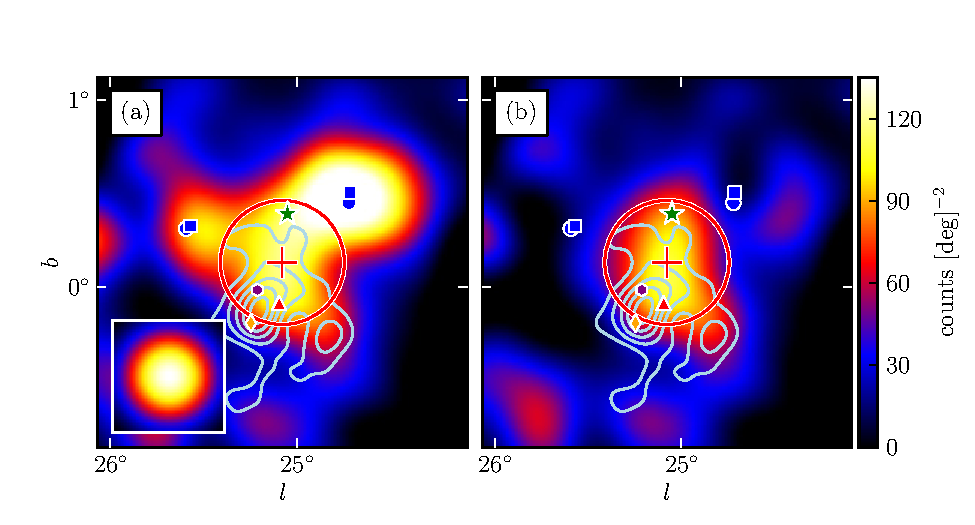
\includegraphics{source_plots/source_HESS_J1837-069_color.pdf}
  \caption{A diffuse-emission-subtracted 10 \gev to 100 \gev counts map
  of the region around 2FGL\,J1837.3$-$0700c (a) smoothed by a 0\fdg15
  2D Gaussian kernel and (b) with the emission from the background
  sources subtracted.  The triangular marker (colored red in the online
  version) represents the 2FGL position of this source.  The plus-shaped
  marker and the circle (colored red) represent the best fit position
  and extension of 2FGL\,J1837.3$-$0700c assuming a radially-symmetric
  uniform disk model.  The circular and square-shaped markers (colored
  blue) represent the 2FGL and the relocalized positions respectively
  of two background 2FGL sources subtracted in (b).  The star-shaped
  marker (colored green) represents 2FGL\,J1835.5$-$0649, another 2FGL
  source that was removed from the background model.  The contours
  (colored light blue) correspond to the \tev image of HESS\,J1837$-$069
  \citep{aharonian_2006a_h.e.s.s.-survey}.  The diamond-shaped marker
  (colored orange) represents the position of PSR\,J1838$-$0655 and
  the hexagonal-shaped marker (colored purple) represents the position
  AX\,J1837.3$-$0652 \citep{gotthelf_2008a_discovery-young}.}
  \figlabel{1FGL_J1837.5-0659c}
\end{figure}

2FGL\,J1837.3$-$0700c was found by our search to be an extended source
candidate in the 10 \gev to 100 \gev energy range and is spatially
coincident with the \tev source HESS\,J1837$-$069.  This source
is in a complicated region.  \figref{1FGL_J1837.5-0659c}a shows a
smoothed counts map of the region and overlays the \tev contours of
HESS\,J1837$-$069 \citep{aharonian_2006a_h.e.s.s.-survey}.  There
are two very nearby point-like 2FGL sources, 2FGL\,J1836.8$-$0623c
and 2FGL\,J1839.3$-$0558c, that clearly represent distinct sources.
On the other hand, there is another source 2FGL\,J1835.5$-$0649 located
between the three sources that appears to correlate with the \tev
morphology of HESS\,J1837$-$069 but at \gev energies does not appear
to represent a physically distinct source.  We concluded that this
source was included in the 2FGL catalog to compensate for residuals
induced by not modeling the extension of this source and removed
it from our model of the sky.  \figref{1FGL_J1837.5-0659c}b shows a
counts map of this region after subtracting these background sources.
After removing 2FGL\,J1835.5$-$0649, we tested for source confusion
by fitting 2FGL\,J1837.3$-$0700c instead as two point-like sources.
Because $\tsinc=10.8$ is less than $\tsext=18.5$, we conclude that this
emission does not originate from two nearby point-like sources.

With this model, 2FGL\,J1837.3$-$0700c was found to have an extension
$\sigma=0\fdg33\pm0\fdg07_\stat\pm0\fdg05_\sys$.  While fitting
the extension of 2FGL\,J1837.3$-$0700c, we iteratively relocalized
the two closest background sources along with the extension of
2FGL\,J1837.3$-$0700c but their positions did not significantly
change.  2FGL\,J1834.7$-$0705c moved to $(l,b)=(24\fdg77,0\fdg50)$,
2FGL\,J1836.8$-$0623c moved to $(l,b)=(25\fdg57,0\fdg32)$.

\ac{HESS} measured an extension of $\sigma=0\fdg12\pm0\fdg02$ and
$0\fdg05\pm0\fdg02$ of the coincident \tev source HESS\,J1837$-$069
along the semi-major and semi-minor axis when fitting this source with
an elliptical 2D Gaussian surface brightness profile.  This corresponds
to a 68\% containment radius of $\rsixeight=0\fdg18\pm0\fdg03$ and
$0\fdg08\pm0\fdg03$ along the semi-major and semi-minor axis. The size
is not significantly different from the LAT 68\% containment radius of
$\rsixeight=0\fdg27\pm0\fdg07$ (less than $2\sigma$).  \figref{hess_seds}
shows that the spectrum of 2FGL\,J1837.3$-$0700c at \gev energies connects
to the spectrum of HESS\,J1837$-$069 at \tev energies.

HESS\,J1837$-$069 is coincident with the hard and steady X-ray source
AX\,J1838.0$-$0655 \citep{bamba_2003a_diffuse-x-ray}.  This source
was discovered by RXTE to be a pulsar (PSR J1838-0655) sufficiently
luminous to power the \tev emission and was resolved by \chandra
to be a bright point-like source surrounded by a $\sim2\arcmin$
nebula \citep{gotthelf_2008a_discovery-young}. The $\gamma$-ray
emission may be powered by this pulsar.  The hard spectral index
and spatial extension of 2FGL\,J1837.3$-$0700c disfavor a pulsar
origin of the LAT emission and suggest instead that the \gev and \tev
emission both originate from the pulsar's wind.  There is another
X-ray point-like source AX\,J1837.3$-$0652 near HESS\,J1837$-$069
\citep{bamba_2003a_diffuse-x-ray} that was also resolved into a point-like
and diffuse component \citep{gotthelf_2008a_discovery-young}.  Although no
pulsations have been detected from it, it could also be a pulsar powering
some of the $\gamma$-ray emission.

\subsection{2FGL\,J2021.5+4026}
\subseclabel{section_2FGL_J2021.5+4026}

The source 2FGL\,J2021.5+4026 is associated with the $\gamma$-Cygni
SNR and has been speculated to originate from the interaction
of accelerated particles in the SNR with dense molecular clouds
\citep{pollock_1985a_probable-identification,gaisser_1998a_gamma-ray-production}.
This association was disfavored when the \gev
emission from this source was detected to be pulsed
\citep[PSR\,J2021+4026,][]{abdo_2010a_first-fermi}.  This pulsar was
also observed by AGILE \citep{chen_2011a_study-gamma-ray}.

\begin{figure}[htbp]
  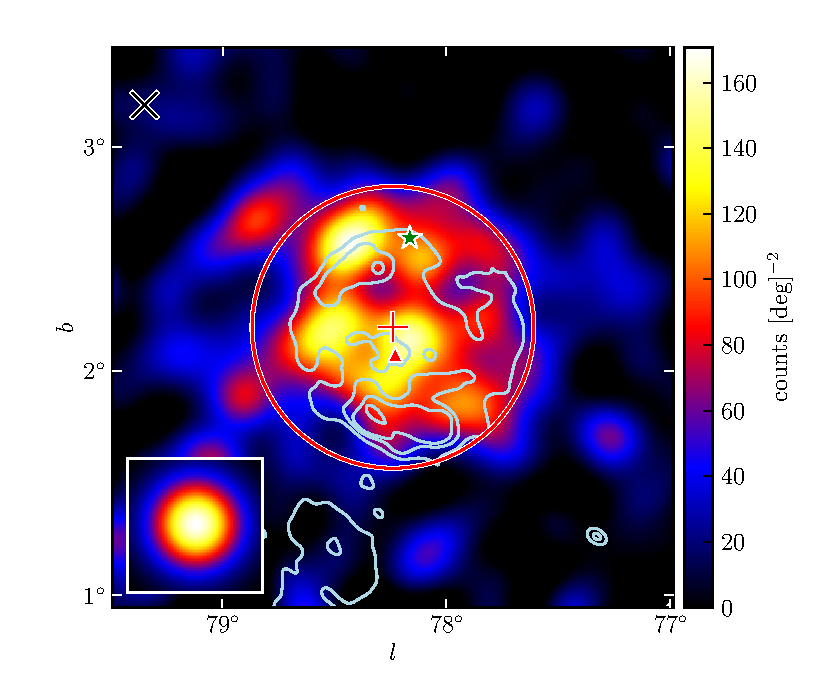
\includegraphics{source_plots/source_Gamma_Cygni_color.pdf}
  \caption{A diffuse-emission-subtracted 10 \gev to 100 \gev counts
  map of the region around 2FGL\,J2021.5+4026 smoothed by a 0\fdg1
  2D Gaussian kernel. The triangular marker (colored red in the
  online version) represents the 2FGL position of this source.
  The plus-shaped marker and the circle (colored red) represent the
  best fit position and extension of 2FGL\,J2021.5+4026 assuming
  a radially-symmetric uniform disk model.  The star-shaped marker
  (colored green) represents 2FGL\,J2019.1+4040, a 2FGL source that was
  removed from the background model.  2FGL\,J2021.5+4026 is spatially
  coincident with the $\gamma$-Cygni SNR.  The contours (colored light
  blue) correspond to the 408MHz image of $\gamma$-Cygni observed by the
  Canadian Galactic Plane Survey \citep{taylor_2003a_canadian-galactic}.}
  \figlabel{1FGL_J2020.0+4049}
\end{figure}

Looking at the same region at energies above 10 \gev, the pulsar is
no longer significant but we instead found in our search an extended
source candidate.  \figref{1FGL_J2020.0+4049} shows a counts map of this
source and overlays radio contours of $\gamma$-Cygni from the Canadian
Galactic Plane Survey \citep{taylor_2003a_canadian-galactic}.  There is
good spatial overlap between the SNR and the \gev emission.

\begin{figure}[htbp]
  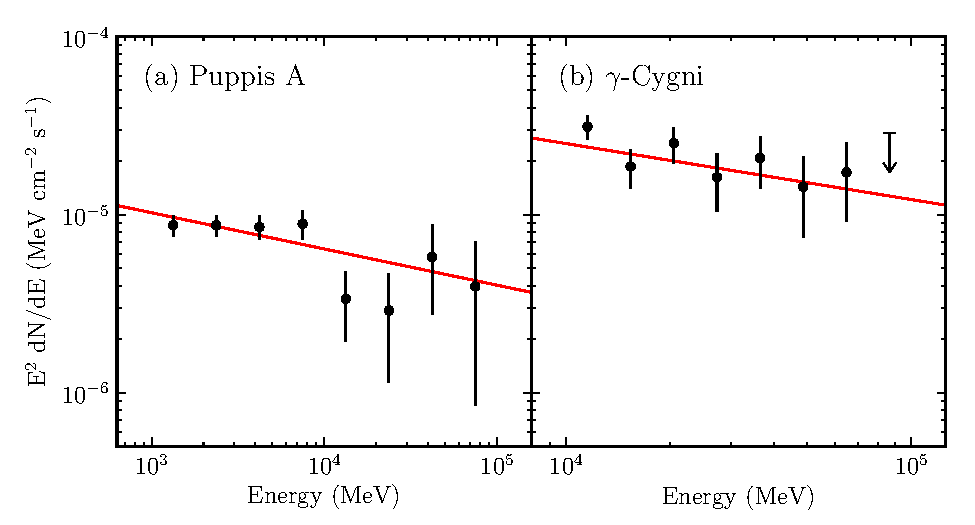
\includegraphics{chapters/extended_search/figures/summary_plots/snr_seds_color.pdf}
  \caption{The spectral energy distribution of the extended sources Puppis
  A (2FGL\,J0823.0$-$4246) and $\gamma$-Cygni (2FGL\,J2021.5+4026).
  The lines (colored red in the online version) are the best fit
  power-law spectral models of these sources. Puppis A has a spectral
  index of $2.21\pm0.09$ and $\gamma$-Cygni has an index of $2.42\pm0.19$.
  The spectral errors are statistical only.  The upper limit is at the
  95\% confidence level.}
  \figlabel{snr_seds}
\end{figure}

There is a nearby source 2FGL\,J2019.1+4040 that correlates with the
radio emission of $\gamma$-Cygni and at \gev energies does not appear
to represent a physically distinct source.  We concluded that it was
included in the 2FGL catalog to compensate for residuals induced by
not modeling the extension of $\gamma$-Cygni and removed it from our
model of the sky.  With this model, 2FGL\,J2021.5+4026 was found to
have an extension $\sigma=0\fdg63\pm0\fdg05_\stat\pm0\fdg04_\sys$
with $\tsext=128.9$.  \figref{snr_seds} shows its spectrum.
The inferred size of this source at \gev energies well
matches the radio size of $\gamma$-Cygni.  Milagro detected a
$4.2\sigma$ excess at energies $\sim 30$ \tev from this location
\citep{abdo_2009a_fermi/large-telescope,abdo_2009a_milagro-observations}.
VERITAS also detected an extended source VER\,J2019+407
coincident with the SNR above 200 \gev and suggested that the
\tev emission could be a shock-cloud interaction in $\gamma$-Cygni
\citep{weinstein_2009a_veritas-survey}.

\section{Discussion}
\seclabel{extended_source_discussion}

\begin{figure}[htbp]
  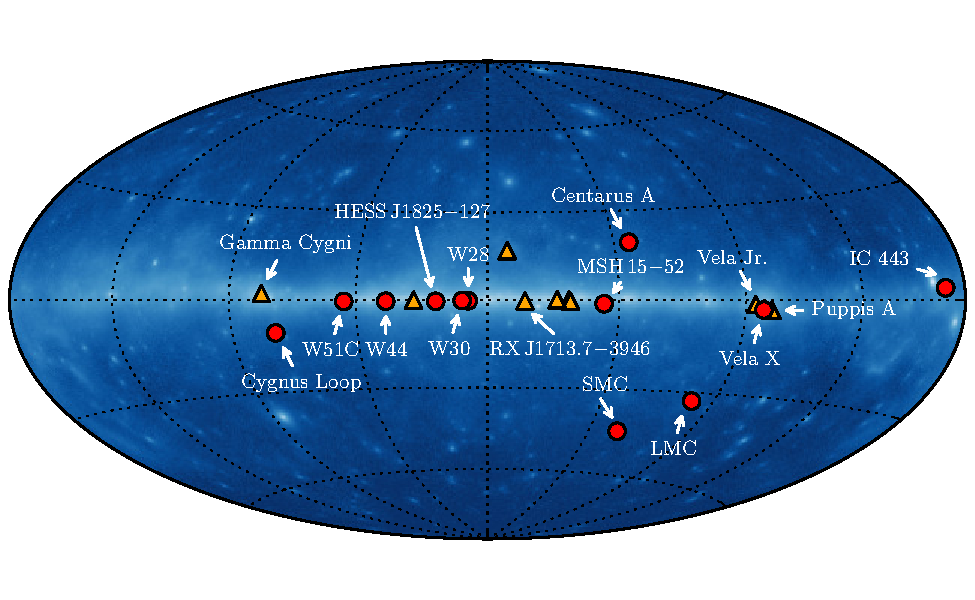
\includegraphics{chapters/extended_search/figures/summary_plots/allsky_extended_sources_color.pdf}
  \caption{The 21 spatially extended sources detected by the LAT at \gev
  energies with 2 years of data.  The twelve extended sources included
  in 2FGL are represented by the circular markers (colored red in the
  online version).  The nine new extended sources are represented by
  the triangular markers (colored orange).  The source positions are
  overlaid on a 100 \mev to 100 \gev Aitoff projection sky map of the
  LAT data in Galactic coordinates.}
  \figlabel{allsky_extended_sources}
\end{figure}

Twelve extended sources were included in the 2FGL catalog and two
additional extended sources were studied in dedicated publications.
Using 2 years of LAT data and a new analysis method, we presented the
detection of seven additional extended sources.  We also reanalyzed the
spatial extents of the twelve extended sources in the 2FGL catalog and
the two additional sources.  The 21 extended LAT sources are located
primarily along the Galactic plane and their locations are shown in
\figref{allsky_extended_sources}.  Most of the LAT-detected extended
sources are expected to be of Galactic origin as the distances of
extragalactic sources (with the exception of the local group Galaxies) are
typically too large to be able to resolve them at $\gamma$-ray energies.

\begin{figure}[htbp]
  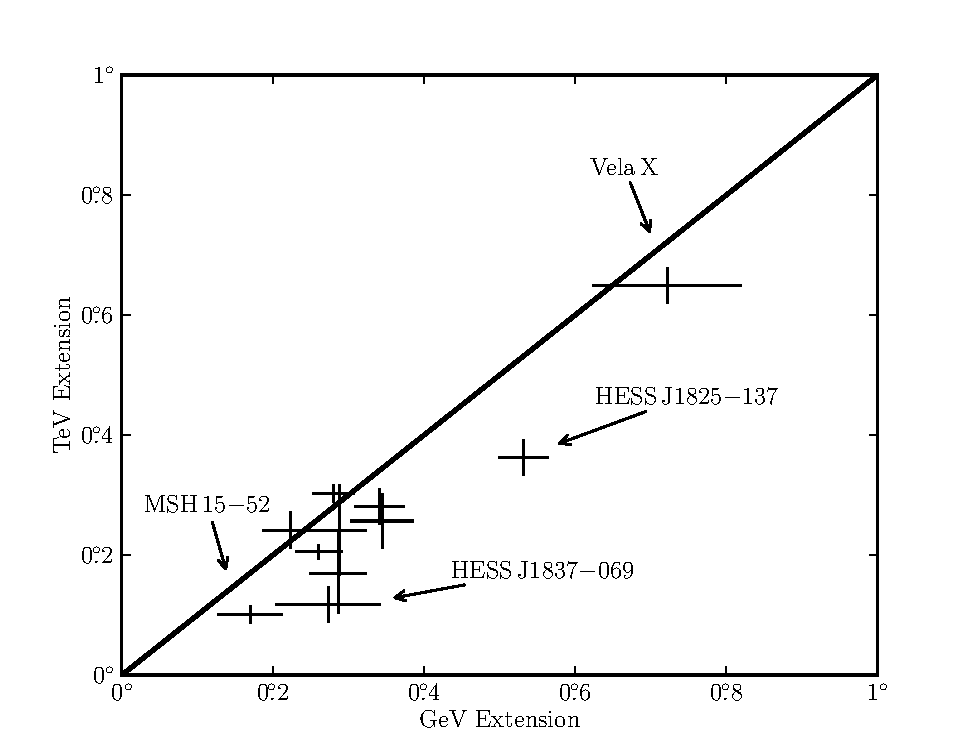
\includegraphics{chapters/extended_search/figures/summary_plots/gev_vs_tev_plot_color.pdf}
  \caption{A comparison of the sizes of extended sources
  detected at both \gev and \tev energies.  The \tev sizes
  of W30, 2FGL\,J1837.3$-$0700c, 2FGL\,J1632.4$-$4753c,
  2FGL\,J1615.0$-$5051, and 2FGL\,J1615.2$-$5138 are from
  \cite{aharonian_2006a_h.e.s.s.-survey}.  The \tev sizes of MSH\,15$-$52,
  HESS\,J1825$-$137, Vela X, Vela Jr., RX\,J1713.7$-$3946 and W28 are from
  \cite{aharonian_2005a_discovery-extended,aharonian_2006a_energy-dependent,aharonian_2006a_first-detection,aharonian_2007a_h.e.s.s.-observations,aharonian_2007a_primary-particle,aharonian_2008a_discovery-energy}.
  The \tev size of IC~443 is from
  \cite{acciari_2009a_observation-extended} and W51C is from
  \cite{krause_2011a_probing-proton}.  The \tev sizes of MSH\,15$-$52,
  HESS\,J1614$-$518, HESS\,J1632$-$478, and HESS\,J1837$-$069 have only
  been reported with an elliptical 2D Gaussian fit and so the plotted
  sizes are the geometric mean of the semi-major and semi-minor axis.  The
  LAT extension of Vela X is from \cite{abdo_2010c_fermi-large}.  The \tev
  sources were fit assuming a 2D Gaussian surface brightness profile so
  the plotted \gev and \tev extensions were first converted to \rsixeight
  (see \subsecref{compare_source_size}).  Because of their large sizes,
  the shape of RX\,J1713.7$-$3946 and Vela Jr.  were not directly fit
  at \tev energies and so are not included in this comparison. On
  the other hand, dedicated publications by the LAT collaboration
  on these sources showed that their morphologies are consistent
  \citep{abdo_2011a_observations-young,tanaka_2011a_gamma-ray-observations}.
  The LAT extension errors are the statistical and systematic errors
  added in quadrature.}
  \figlabel{gev_vs_tev_plot}
\end{figure}

For the LAT extended sources also seen at \tev energies,
\figref{gev_vs_tev_plot} shows that there is a good correlation between
the sizes of the sources at \gev and \tev energies. Even so, the sizes
of PWNe are expected to vary across the \gev and \tev energy range and
the size of HESS\,J1825$-$137 is significantly larger at \gev than \tev
energies \citep{grondin_2011a_detection-pulsar}.  It is interesting to
compare the sizes of other PWN candidates at \gev and \tev energies, but
definitively measuring a difference in size would require a more in-depth
analysis of the LAT data using the same elliptical Gaussian spatial model.

\begin{figure}[htbp]
  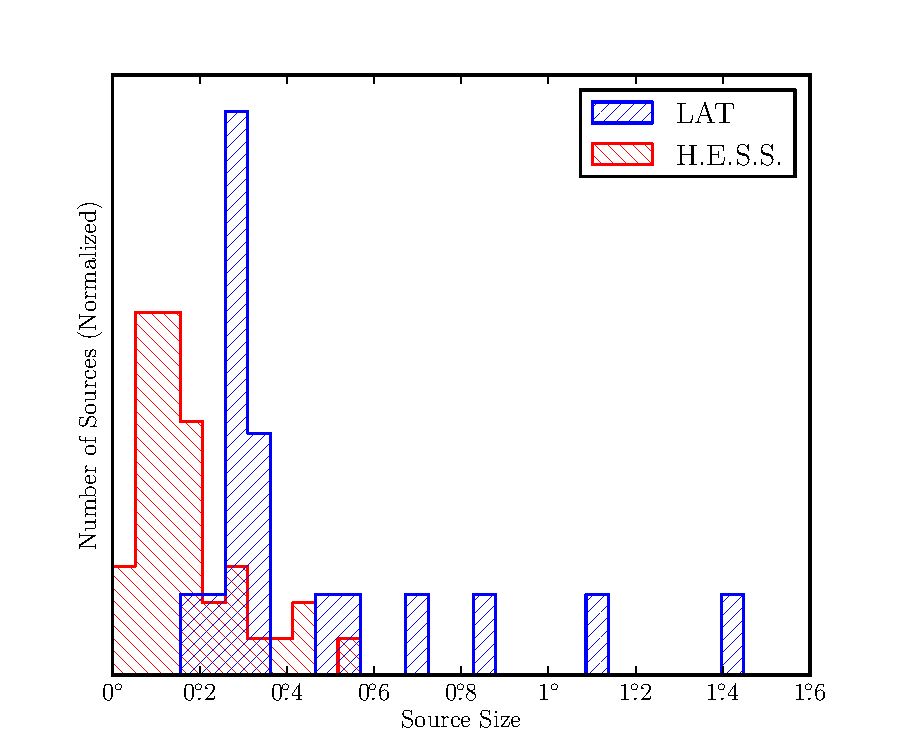
\includegraphics{chapters/extended_search/figures/summary_plots/gev_vs_tev_histogram_color.pdf}
  \caption{The distributions of the sizes of 18 extended LAT sources at
  \gev energies (colored blue in the electronic version) and the sizes of
  the 40 extended \ac{HESS} sources at \tev energies (colored red).  The
  \ac{HESS} sources were fit with a 2D Gaussian surface brightness profile
  so the LAT and \ac{HESS} sizes were first converted to \rsixeight.
  The \gev size of Vela X is taken from \cite{abdo_2010c_fermi-large}.
  Because of their large sizes, the shape of RX\,J1713.7$-$3946 and Vela
  Jr. were not directly fit at \tev energies and are not included in this
  comparison.  Centaurus A is not included because of its large size.}
  \figlabel{gev_vs_tev_histogram}
  \end{figure}

\figref{gev_vs_tev_histogram} compares the sizes of the 21 extended LAT
sources to the 42 extended \ac{HESS} sources.\footnote{The \tev extension
of the 42 extended \ac{HESS} sources comes from the \ac{HESS} Source
Catalog \url{http://www.mpi-hd.mpg.de/hfm/HESS/pages/home/sources/}.}
Because of the large field of view and all-sky coverage, the LAT can
more easily measure larger sources.  On the other hand, the better
angular resolution of \acp{IACT} allows them to measure a population
of extended sources below the resolution limit of the LAT (currently
about $\sim0\fdg2$).  \fermi has a 5 year nominal mission lifetime with
a goal of 10 years of operation.  As \figref{time_sensitivity} shows,
the low background of the LAT at high energies allows its sensitivity
to these smaller sources to improve by a factor greater than the square
root of the relative exposures.  With increasing exposure, the LAT will
likely begin to detect and resolve some of these smaller \tev sources.

\begin{figure}[htbp]
  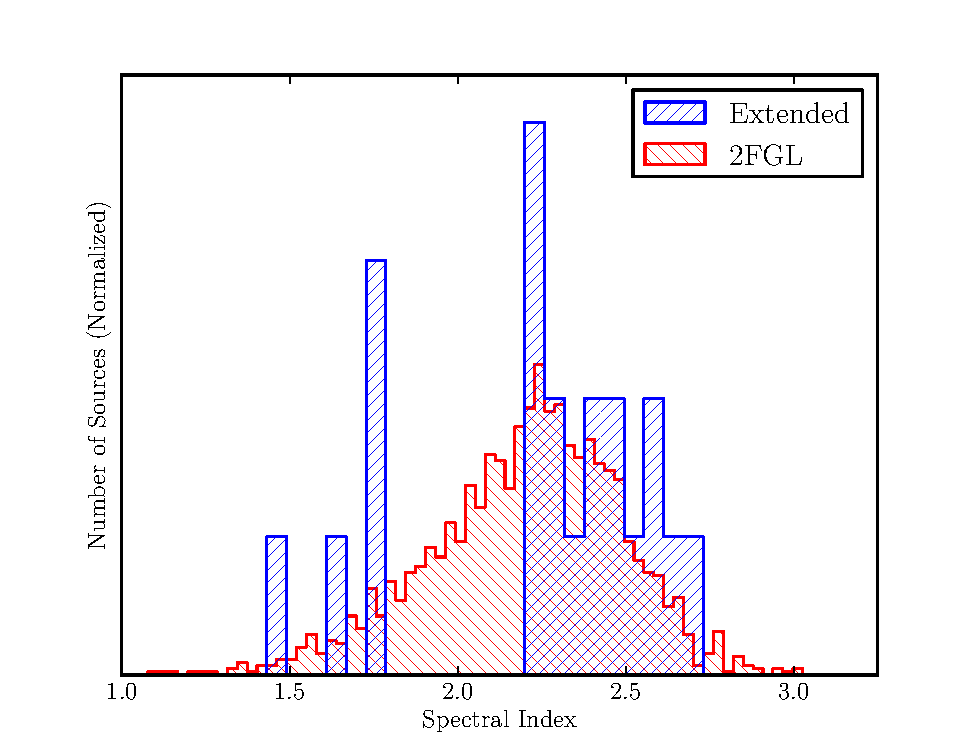
\includegraphics{chapters/extended_search/figures/summary_plots/compare_index_2FGL_color.pdf}
  \caption{The distribution of spectral indices of the 1873 2FGL sources
  (colored red in the electronic version) and the 21 spatially extended
  sources (colored blue).  The index of Centaurus A is taken from
  \cite{nolan_2012_fermi-large} and the index of Vela X is taken from
  \cite{abdo_2010c_fermi-large}.}
  \figlabel{compare_index_2FGL}
\end{figure}

\figref{compare_index_2FGL} compares the spectral indices of LAT
detected extended sources and of all sources in the 2FGL catalog. This,
and \tabref{known_extended_sources} and \tabref{new_ext_srcs_table},
show that the LAT observes a population of hard extended sources at
energies above 10 \gev.  \figref{hess_seds} shows that the spectra of
four of these sources (2FGL\,J1615.0$-$5051, 2FGL\,J1615.2$-$5138,
2FGL\,J1632.4$-$4753c, and 2FGL\,J1837.3$-$0700c) at \gev energies
connects to the spectra of their \ac{HESS} counterparts at
\tev energies. This is also true of Vela Jr., HESS\,J1825$-$137
\citep{grondin_2011a_detection-pulsar}, and RX\,J1713.7$-$3946
\citep{abdo_2011a_observations-young}.  It is likely that the \gev and
\tev emission from these sources originates from the same population of
high-energy particles.

Many of the \tev-detected extended sources now seen at \gev energies
are currently unidentified and further multiwavelength follow-up
observations will be necessary to understand these particle accelerators.
Extending the spectra of these \tev sources towards lower energies with
LAT observations may help to determine the origin and nature of the
high-energy emission.


\chapter{Search for \Acsptitle{PWN} Associated with Gamma-loud Pulsars}
\chaplabel{offpeak}

\paperref{
  This chapter is based on section seven ``Unpulsed Magnetospheric Emission'' from  
  the paper ``The Second \fermi Large Area Telescope Catalog of Gamma-ray Pulsars''
  \citep{abdo_2013a_second-fermi}.}

Some pulsars have magnetospheric emission over their full rotation phase
with similar spectral characteristics to the emission seen through
their peaks.  This emission appears in the observed light curves as
a low-level, unpulsed component above the estimated background level
(i.e., not attributable to diffuse emission or nearby point sources)
and can be a powerful discriminator for the emission models.

On the other hand a PWN around the pulsar, or a photon excess due
to imprecise knowledge of diffuse emission around the pulsar, would
not be modulated at the rotational period and could be confused with
a constant magnetospheric signal.  Including the discovery of the GeV
PWN 3C 58 associated with PSR J0205+6449 described in this section, the
LAT sees 17 sources potentially associated with PWNe at GeV energies
\citep{acero_2013a_constraints-galactic}.  Some are highlighted in
\secref{off_peak_individual_source_discussion}.  This off-peak emission
should be properly modeled when searching for pulsar emission at all
rotation phases.

We can discriminate between these two possible signals through
spectral and spatial analysis.  If the emission is magnetospheric,
it is more likely to appear as a non-variable point source with
an exponentially cutoff spectrum with a well-known range of cutoff
energies.  On the other hand, PWNe and diffuse excesses have spectra
with a power-law shape and either a hard index continuing up to tens
of GeV in the PWN case or present only at lower energies with a very
soft index in the diffuse case.  In addition, PWNe are often spatially
resolvable at GeV energies \citep[e.g., Vela-X has been spatially
resolved with the LAT and \textit{AGILE} and HESS J1825$-$137 with the
LAT;][respectively]{abdo_2010c_fermi-large,pellizzoni_2010a_detection-gamma-ray,grondin_2011a_detection-pulsar}
so an extended source would argue against a magnetospheric origin of the
emission.  However, given the finite angular resolution of the LAT not all
PWNe will appear spatially extended at GeV energies.  The Crab Nebula,
for instance, cannot be resolved by the LAT but can be distinguished
from the gamma-bright Crab pulsar, in the off-peak interval, by its hard
spectrum above $\sim$1 GeV \citep{abdo_2010a_fermi-large}.  In addition,
GeV emission from the Crab Nebula was discovered to be time-variable
\citep[e.g.,][]{abdo_2011a_gamma-ray-flares} providing another possible
way to discern the nature of any observed off-peak signal.


Therefore, to identify pulsars with magnetospheric emission across
the entire rotation, we define and search the off-peak intervals
of the pulsars in this catalog for significant emission, except PSR
J2215+5135 for which the rotation ephemeris covers a short time interval
and the profile is noisy.  We then evaluate the spectral and spatial
characteristics of any off-peak emission to determine if it is likely
magnetospheric, related to the pulsar wind, or physically unrelated to
the pulsar (e.g., unmodeled diffuse emission).

\section{Off-peak Phase Selection}
\seclabel{peak_definition}

We first developed a systematic, model-independent, and computationally-efficient method 
to define the off-peak interval of a pulsar light curve.

We begin by deconstructing the light curve 
into simple Bayesian Blocks using the algorithm described in
\citet{jackson_2005a_algorithm-optimal} and \citet{scargle_2013a_studies-astronomical}.  
We could not apply the Bayesian Block algorithm to the weighted-counts
light curves because they do not follow Poisson statistics, required
by the algorithm.
We therefore use an unweighted-counts light curve in which the angular radius and minimum energy selection have been varied to maximize the H-test statistic.  To produce Bayesian Blocks on a periodic light curve,
we extend the data over three rotations, by copying and shifting the
observed phases to cover the phase range from $-$1 to 2.  We do, however,
define the final blocks to be between phases 0 and 1.  
To avoid potential contamination from the trailing or leading edges of
the peaks, we reduce the extent of the block by 10\% on either side,
referenced to the center of the block.

There is one free parameter in the Bayesian Block algorithm called
ncp$\rm _{prior}$ which modifies the probability that the
algorithm will divide a block into smaller intervals.
We found that, in most cases, setting ncp$\rm _{prior}=8$ protects against
the Bayesian Block decomposition containing unphysically small blocks.
For a few marginally-detected pulsars, the algorithm failed 
to find more than one block and we had to decrease ncp$\rm _{prior}$ until the
algorithm found a variable light curve. Finally, for a few pulsars the 
Bayesian-block decomposition of the light curves failed to model 
weak peaks found by the light-curve fitting method
presented in \secref{lightCurveFitting} or extended
too far into the other peaks. For these pulsars,
we conservatively shrink the off-peak region.

For some pulsars, the observed light curve has two well-separated peaks
with no significant bridge emission, which leads to two well-defined
off-peak intervals.  We account for this possibility by finding the second-lowest 
Bayesian block and accepting it as a second off-peak interval if
the emission is consistent with that in the lowest block (at the 99\%
confidence level) and if the extent of the second block is at least half
that of the first block.

Figure~\ref{off_peak_select} shows the energy-and-radius optimized
light curves, the Bayesian block decompositions, 
and the off-peak intervals for six pulsars.  
Figures \ref{J0034-0534lc} to \ref{J2240+5832lc} overlay off-peak intervals
over the weighted light curves of several pulsars.
The off-peak
intervals for all pulsars in this catalog are given in Tables \ref{tbl-pulsePSR} and \ref{tbl-pulseMSP}.

\begin{figure}
  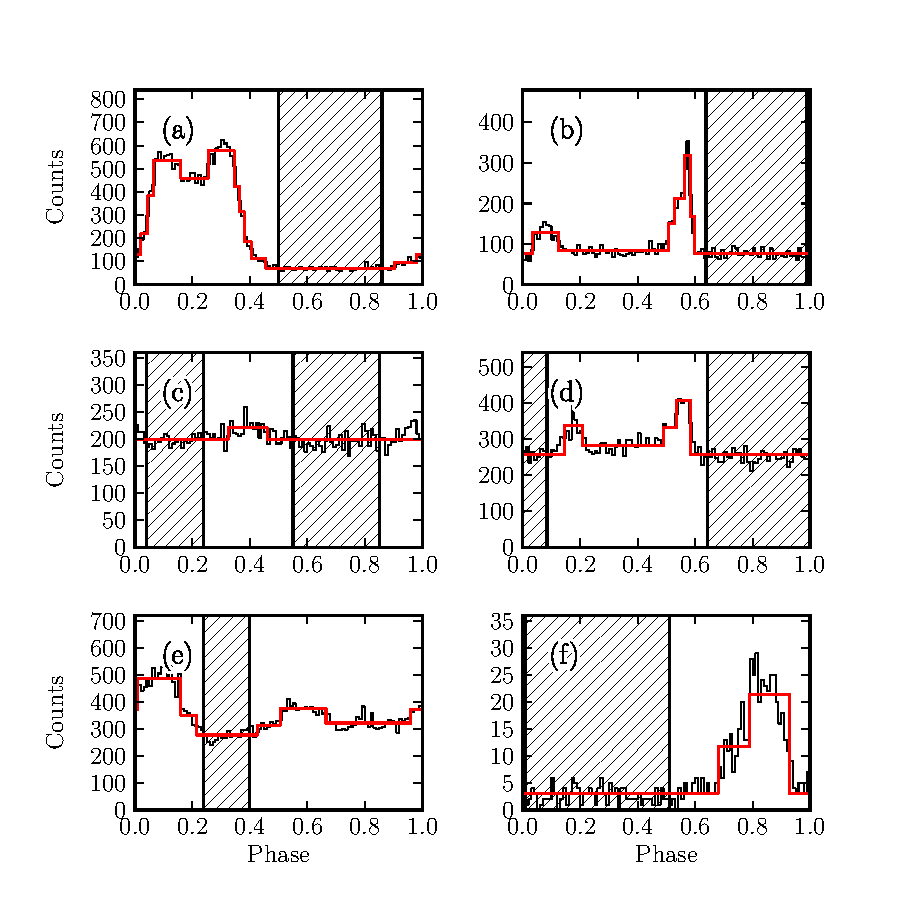
\includegraphics{chapters/offpeak/figures/off_peak_phase_color.pdf}
  \caption{The energy-and-radius optimized light curve, Bayesian block decomposition of the        
  light curve, and off-peak interval for
  (a) PSR J0007+7303, (b) PSR J0205+6449, (c) PSR J1410$-$6132,
  (d) PSR J1747$-$2958, (e) PSR J2021+4026, and (f) PSR J2124$-$3358.
  The black histograms represent the light curves,
  the gray lines (colored red in the electronic version)
  represent the Bayesian block decompositions of the pulsar light curves, and
  the hatched areas represent the off-peak intervals selected by this method.}
  \figlabel{off_peak_select}
\end{figure}


\subsection{Off-peak Analysis Method}
\label{off_peak_analysis}

Characterizing both the spatial and spectral
characteristics of any off-peak emission helps discern its origin.
We employ a somewhat different analysis procedure here than
for the phase-averaged analysis described in Section
\ref{spectralMethodSection}.  To evaluate the spatial characteristics of
any off-peak emission we use the likelihood fitting package \pointlike
\citep[detailed in][]{LAT_collaboration_extended_search_2012}, and
to fit the spectrum we use \gtlike in binned mode via {\it pyLikelihood} as was done for the
phase-averaged analysis.

For each pulsar we start from
the same temporal and spatial event selections described in Section
\ref{obsvSection} but we increase the maximum energy to 400 GeV (the
highest event energy for any ROI under this selection is $\sim$316 GeV).
For the \pointlike analysis we further select a 10$\degree$ radius ROI
and for \gtlike a $14\degree\times14\degree$ square ROI, both centered
on the pulsar postition.  Finally, we only consider photons with 
pulse phases within the corresponding off-peak interval.

We search for off-peak emission
assuming a point source and (except for the Crab Nebula and Vela-X, described below) 
a power-law spectral model.  We fit the position of this
putative off-peak source using \pointlike as described by \citet{2FGL}
and then use the best-fit position in a spectral analysis with \gtlike.
From the spectral analysis we require $TS\geq25$ (just over $4\sigma$)
to claim a detection.  If $TS<25$, we compute upper limits on the flux 
in the energy range from 100 \mev to 316 \gev
assuming
a power law with photon index fixed to 2.0 and a PLEC1 model with
$\Gamma=1.7$ and $E_{\rm cut}=3$ GeV.

The spectrum of the Crab Nebula (associated with PSR J0534+2200) is
uniquely challenging because the GeV spectrum contains both a falling
synchrotron and a rising inverse Compton component \citep{FermiCrab}.
For this particular source we used the best-fit two-component spectral
model from \cite{LAT_collaboration_crab_2012} and fit only the overall
normalization of the source. 
In addition, for Vela-X (associated with PSR J0835-4510) we took the
best-fit spectral model from \cite{FermiVelaX2nd} and fit only the overall
normalization of this source. This spectrum has a smoothly broken power
law spectral model and was fit assuming Vela-X to have an elliptical
disk spatial model.

If the off-peak source is significant, we test whether the spectrum shows
evidence for a cutoff, as described in Section \ref{spectralMethodSection}
and by \citet{LAT_collaboration_PWNCAT_2011}, assuming the source is at
the pulsar position.  We say that the off-peak emission shows evidence for
a cutoff if $TS_{\rm cut}\geq9$, corresponding to a $3\sigma$ detection.

For a significant off-peak point source,
we use \pointlike to test if the emission is significantly
extended.  We assume a radially-symmetric Gaussian source
and fit the position and extension parameter ($\sigma$) as described
in \citet{LAT_collaboration_extended_search_2012}.  The best-fit
extended source parameters are then given to \gtlike, which is used
to fit the spectral parameters and the significance of the extension
over a point source, $TS_{\rm ext}$, evaluated as described in
\citet{LAT_collaboration_extended_search_2012}.  
That paper established that $TS_{\rm ext}\geq16$ means highly probable source extension.
In the present work we aim only to flag possible extension, and use  $TS_{\rm ext}\geq9$.
%% 
%% We say that the off-peak emission shows evidence for extension if $TS_{\rm ext}\geq16$.

To test for variability, even without significant emission over the 3-year time
range, we divide the dataset into 36 intervals and fit the point-source
flux independently in each interval, 
computing $TS_{\rm var}$ as in 2FGL.  
For sources with potential magnetospheric off-peak emission and for
regions with no detection, we performed the test at the pulsar's position.
Otherwise, we test at the best-fit position.
The off-peak emission is said
to show evidence for variability if $TS_{\rm var}\geq91.7$, corresponding
to a $4\sigma$ significance.  
%
As noted in Section \ref{obsvSection}, our timing solutions for PSRs J0205+6449 and J1838$-$0537 are not  
coherent across all three years.  
For these two pulsars, we excluded the time ranges without ephemerides  
and only tested for variability during months that were completely covered.  
For J1838$-$0537 only one month is lost, whereas for J0205+6449 the 7\% data loss is spread across
three separate months.
As a result, $TS_{\rm var}$ for these pulsars is a conservative estimate of variability significance.

The procedure described above, especially the extension analysis,
is particularly sensitive to sources not included in 2FGL that are near the pulsar of interest,
for two reasons.
First, we are using an additional year of data and second,
when ``turning off'' a bright pulsar nearby, faint sources become more
important to the global fit.  Therefore, in many situations we had to run
the analysis several times, iteratively improving the model by including
new sources, until we removed all $TS>25$ residuals. The final
\gtlike-formatted XML source model for each off-peak 
region is included in the auxiliary material.

There are still, however, pulsars for which we were unable to obtain
an unbiased fit of the off-peak emission,
most likely due to inaccuracies in the model of the Galactic diffuse emission
and incorrectly modeled nearby sources.  The most common symptom
of a biased fit is an unphysically large extension.  In these cases,
the extended source attempts to account for multiple point sources or
incorrectly-modeled diffuse emission,
not just the putative off-peak emission.  Systematics associated
with modeling extended sources are discussed more thoroughly in
\citet{LAT_collaboration_extended_search_2012}.  For the purposes of this
catalog, we have flagged the pulsars where off-peak analysis suffered from
these issues and do not attempt a complete understanding of the emission.

Observations of magnetospheric off-peak emission can be used to 
constrain pulsar geometry. Therefore, it is important to know if 
off-peak emission that is otherwise pulsar-like might instead
be incorrectly-modeled Galactic diffuse emission. 
We therefore performed a limited study of the systematics
associated with our model of the Galactic diffuse emission.

For sources which otherwise would be classified as magnetospheric, we
tested the significance of the emission assuming eight different
Galactic diffuse emission models as described in \citet{SNRCatDiffuseSystematics}. 
These models were constructed using a different model building strategy,
vary parameters of the Galactic diffuse emission model, and
have additional degrees of freedom in the fit.

We define $\tsaltdiff$ as the minimum test statistic of any of the
eight alternate diffuse models. This test statistic is computed
assuming the emission to be pointlike at the best-fit position
and is therefore comparable to \tspoint.
For sources which would otherwise be considered magnetospheric,
we flag the emission as potentially 
spurious if $\tsaltdiff<25$.
We caution that although this test can help to 
flag problematic regions,
these models do not probe the entirety of the uncertainty
associated with our model of the Galactic diffuse emission.
Therefore, some diffuse emission could still be incorrectly classified
as magnetospheric.


\subsection{Off-peak Results}
\subseclabel{off_peak_results}

The off-peak intervals of 54 LAT-detected pulsars have
been evaluated by \citet{LAT_collaboration_PWNCAT_2011} using 16 months of sky survey observations.  
This led to the discovery of PWN-like emission
in the off-peak interval of PSR J1023$-$5746, coincident with HESS
J1023$-$575, and identification of 5 pulsars that appear to have near 100\%
duty cycles.  Our results, summarized in Table \ref{tbl-off_peak_table},
extend the analysis to 116 pulsars over 3 years of data.  
Sample off-peak spectra are shown in Figure \ref{off_peak_seds}.
Using the procedures outlined in Sections \ref{peak_definition}
and \ref{off_peak_analysis}, we have identified 34 pulsars that
have significant emission ($TS\geq25$) in their off-peak intervals.
We classify the likely nature of the emission as follows.

If the emission has $TS_{\rm cut}\geq9$, we consider the emission to be
either magnetospheric (`M') or possibly magnetospheric (`M*').
As was discussed in Section \ref{off_peak_analysis}, 
we flag the emission as `M*' if the source is formally spatially extended
($TS_{\rm ext}>16$) or if the source is not robust against varying
the diffuse emission models ($\tsaltdiff<25$). 
On consideration of the angular extent of the PSF of the LAT and inaccuracies in the Galactic diffuse
emission model, we caution against considering the `M*' sources to be definitively classified.
If the source is significantly cutoff, not
significantly extended, and is significant when varying the alternative diffuse models,
we classify the emission as `M'.


On the other hand, if the
emission has $TS_{\rm ext}\geq16$, and does not suffer from confusion as
discussed at the end of Section \ref{off_peak_analysis}, and/or has a hard
photon index, we say it is likely
to originate in the pulsar wind and identify these sources as type `W'.
The remaining sources with off-peak emission not satisfying any of the
previous criteria are identified as type `U' to indicate that the nature
of the emission is unidentified and we do not speculate about its origin.


We identify 9 type `M' sources,
significantly expanding the number of pulsars that perhaps have detectable magnetospheric emission across all rotational phases. 
One caution is that many of these `M' pulsars, especially the young objects, are in regions of particularly bright diffuse gamma-ray
emission, where small fractional uncertainties in the level of diffuse emission can account for much of the apparent unpulsed emission. 
However, if established as true magnetospheric components, these will be important test cases for
pulsar emission models. In addition, we identify ten
`M*'-type regions.
For type `M' and `M*' sources, we present the best-fit spectral parameters using
a point source at the pulsar's position with a PLEC1 spectral model in
%columns 6, 7, and 8 of
Table \ref{tbl-off_peak_table}.  For all other
sources (except the Crab Nebula described in Sec. \ref{off_peak_analysis}), 
we present the spectral results using a power-law spectral
model and the best-fit spatial representation.


Additionally, we identified four off-peak emissions consistent with a PWN
hypothesis, one of them being a new detection at GeV energies (PSR J0205+6449).
Only one of these four, the previously identified Vela$-$X PWN \citep{LAT_collaboration_Vela_X_2010}, is spatially extended for the LAT.
Similarly, we detect six type `U' regions. Three of these are formally 
spatially extended
but because of the spatial systematics 
we assume point-like emission for the spectral analysis.

We mention that for a few sources, the spectral analysis
performed here is in disagreement with the analysis presented in
\citet{LAT_collaboration_PWNCAT_2011}. For soft and faint sources
(including J1044$-$5737 and J1809$-$2332), the spectral discrepancy is
mainly caused by our use of a newer Galactic diffuse model. At lower
energies, small changes in the diffuse model can have a significant
impact on the analysis of a region.  For bright magnetospheric sources
(including J0633+1746 and J2021+4026), the spectral discrepancy is mainly
due to using different phase ranges (see Sec.~\ref{peak_definition}).


\figref{off_peak_luminosity_vs_edot} shows that only
a small fraction of the spindown power goes into 
the gamma-ray emission from LAT-detected PWNe.
Similarly, 
Figure~\ref{P0_sqEDOTD2} shows that the LAT only detects
PWNe from the youngest pulsars with the highest spindown power.
GeV emission from the Crab Nebula is highly time variable (Section \ref{off_peak_analysis}).  
Indeed, we find
$TS_{\rm var}=373$ for the Crab Nebula; however
no other source demonstrated flux variability (all have $16 <TS_{\rm var} <65)$.  
Other GeV PWNe may be variable, but the combination of lower fluxes
and less-extreme variations limits our ability identify them as such.


The off-peak results for several interesting sources are
presented in Appendix~\ref{App-off_peak_individual_source_discussion}.
The complete off-peak search results can be found in the accompanying
auxiliary information described in Appendix \ref{off_peak_auxiliary}.
For regions where we find $TS<25$, the auxiliary information contains
upper limits computed for both a power-law spectral model and a
PLEC1 model with $E_{\rm cut}=3$ GeV and $\Gamma=1.7$.  The auxiliary
information also contains $TS_{\rm var}$ for each off-peak interval.



\begin{deluxetable}{ll*{8}c}
\tablecolumns{8}
\tablewidth{0pt}
\tabletypesize{\scriptsize}
\tablecaption{Off-Peak Spatial and Spectral Results
\label{tbl-off_peak_table}
}
\tablehead{\colhead{PSR} & \colhead{Type} & \colhead{$\tspoint$} & \colhead{$\tsext$} & \colhead{$\tscutoff$} & \colhead{$\tsaltdiff$} & \colhead{Energy Flux} & \colhead{$\Gamma$} & \colhead{$\Ecutoff$}\\ \colhead{ } & \colhead{ } & \colhead{ } & \colhead{ } & \colhead{ } & \colhead{ } & \colhead{($10^{-11}\,\efluxunits$)} & \colhead{ } & \colhead{(GeV)}}
\startdata
\multicolumn{8}{c}{Young Pulsars} \\[3pt]
\hline
J0007+7303 & U & 71.4 & 10.8 & 0.0 &  & $1.98 \pm 0.26$ & $2.61 \pm 0.14$ &  \\
J0205+6449 & W & 33.7 & 0.5 & 0.0 &  & $1.75 \pm 0.68$ & $1.61 \pm 0.21$ &  \\
J0534+2200 & W & 5247. & 0.0 & 0.3 &  & $67.2 \pm 1.6$ & \tablenotemark{a} &  \\
J0631+1036 & U & 33.1 & 0.0 & 5.4 &  & $1.70 \pm 0.33$ & $2.38 \pm 0.14$ &  \\
J0633+1746 & M & 3666. & 2.3 & 239. & 3369. & $41.4 \pm 1.1$ & $1.37 \pm 0.09$ & $0.93 \pm 0.10$ \\
J0734$-$1559 & M* & 28.3 & 12.4 & 30.8 & 0.0 & $1.61 \pm 0.24$ & $0.01 \pm 0.08$ & $0.17 \pm 0.03$ \\
J0835$-$4510 & W & 473. & 283. & 22.8 &  & $30.3 \pm 1.2$ & \tablenotemark{b} &  \\
J0908$-$4913 & M* & 65.1 & 41.4 & 60.4 & 3.1 & $3.04 \pm 1.07$ & $0.15 \pm 0.59$ & $0.30 \pm 0.01$ \\
J1023$-$5746 & M* & 59.7 & 30.0 & 10.9 & 72.5 & $5.35 \pm 1.17$ & $0.57 \pm 0.80$ & $0.49 \pm 0.21$ \\
J1044$-$5737 & M* & 42.0 & 98.1 & 22.4 & 25.6 & $3.12 \pm 0.75$ & $0.80 \pm 0.93$ & $0.40 \pm 0.18$ \\
J1105$-$6107 & M* & 33.3 & 37.5 & 21.7 & 39.4 & $3.81 \pm 0.77$ & $0.92 \pm 0.56$ & $0.48 \pm 0.22$ \\
J1112$-$6103 & U & 65.0 & 71.1 & 0.9 &  & $5.10 \pm 0.74$ & $2.17 \pm 0.09$ &  \\
J1119$-$6127 & U & 61.3 & 1.0 & 0.9 &  & $4.11 \pm 0.63$ & $2.22 \pm 0.09$ &  \\
J1124$-$5916 & M & 95.9 & 0.0 & 18.2 & 59.4 & $2.87 \pm 0.71$ & $1.31 \pm 0.91$ & $1.43 \pm 1.42$ \\
J1410$-$6132 & U & 27.5 & 71.2 & 0.4 &  & $4.29 \pm 1.05$ & $1.90 \pm 0.15$ &  \\
J1513$-$5908 & W & 102. & 3.5 & 0.0 &  & $4.95 \pm 0.83$ & $1.78 \pm 0.12$ &  \\
J1620$-$4927 & M* & 28.9 & 0.5 & 35.2 & 0.0 & $5.25 \pm 0.96$ & $0.35 \pm 0.94$ & $0.57 \pm 0.29$ \\
J1746$-$3239 & M* & 53.3 & 34.3 & 34.2 & 0.0 & $3.65 \pm 0.59$ & $0.94 \pm 0.31$ & $0.60 \pm 0.10$ \\
J1747$-$2958 & M & 45.5 & 5.4 & 49.8 & 50.4 & $8.41 \pm 2.84$ & $0.02 \pm 0.32$ & $0.28 \pm 0.01$ \\
J1809$-$2332 & M* & 32.5 & 13.6 & 21.9 & 0.0 & $4.10 \pm 0.80$ & $0.24 \pm 0.83$ & $0.31 \pm 0.11$ \\
J1813$-$1246 & M & 62.8 & 0.0 & 9.0 & 49.7 & $6.31 \pm 1.40$ & $1.60 \pm 0.73$ & $0.99 \pm 0.95$ \\
J1836+5925 & M & 10407. & 0.0 & 365. & 10401. & $36.9 \pm 0.7$ & $1.47 \pm 0.03$ & $1.98 \pm 0.09$ \\
J1838$-$0537 & M* & 51.3 & 32.9 & 21.9 & 41.9 & $8.35 \pm 1.31$ & $1.39 \pm 0.54$ & $2.55 \pm 2.48$ \\
J2021+4026 & M & 1717. & 8.7 & 244. & 1978. & $64.0 \pm 1.4$ & $1.64 \pm 0.02$ & $1.82 \pm 0.04$ \\
J2032+4127 & U & 53.6 & 76.1 & 1.5 &  & $4.36 \pm 0.77$ & $2.07 \pm 0.12$ &  \\
J2055+2539 & M & 123. & 0.0 & 30.0 & 101. & $1.63 \pm 0.19$ & $1.05 \pm 0.28$ & $0.64 \pm 0.12$ \\
\hline\\[-5pt]
\multicolumn{8}{c}{Millisecond Pulsars} \\[3pt]
\hline
J0034$-$0534 & U & 41.0 & 0.0 & 6.0 &  & $0.82 \pm 0.16$ & $2.40 \pm 0.19$ &  \\
J0102+4839 & U & 49.7 & 0.0 & 7.4 &  & $1.29 \pm 0.20$ & $2.51 \pm 0.14$ &  \\
J0218+4232 & U & 50.1 & 0.0 & 6.8 &  & $2.13 \pm 0.33$ & $2.72 \pm 0.26$ &  \\
J0340+4130 & M* & 26.9 & 0.1 & 16.3 & 11.9 & $0.53 \pm 0.11$ & $0.02 \pm 0.22$ & $0.94 \pm 0.28$ \\
J1658$-$5324 & U & 42.3 & 0.0 & 1.9 &  & $1.69 \pm 0.29$ & $2.52 \pm 0.76$ &  \\
J2043+1711 & U & 52.5 & 0.0 & 8.8 &  & $1.46 \pm 0.27$ & $2.29 \pm 0.14$ &  \\
J2124$-$3358 & M & 129. & 0.0 & 19.8 & 118. & $1.08 \pm 0.15$ & $0.70 \pm 0.51$ & $1.21 \pm 0.49$ \\
J2302+4442 & M & 114. & 0.0 & 9.8 & 105. & $1.45 \pm 0.20$ & $1.54 \pm 0.40$ & $1.61 \pm 0.82$ \\
\enddata


\tablenotetext{a}{The spectral shape of the Crab Nebula was taken from \citet{LAT_collaboration_crab_2012}.}
\tablenotetext{b}{The spectral shape of Vela$-$X was taken from \cite{FermiVelaX2nd}.}

\tablecomments{Off-peak regions with a significant detection of emission.
The source classification is `M' for likely magnetospheric, 
`M*' for possibly magnetospheric but with a problematic spatial analysis or in a region with possibly poorly-modeled
Galactic diffuse emission,
`W' for likely pulsar wind, and `U' for unidentified.
The table includes the significance of the source ($TS$),  
of the source extension ($TS_{\rm ext}$), of a spectral cutoff ($TS_{\rm cut}$),
and with the alternative diffuse models ($\tsaltdiff$). 
The best-fit energy flux and photon index are computed in the energy range from 100 \mev to 316 \gev.
For sources with large $TS_{\rm cut}$, the exponential cutoff energies are presented. 
The quoted errors are statistical only. A few sources are discussed in Section~\ref{off_peak_individual_source_discussion}.
}


\end{deluxetable}

\begin{figure}
  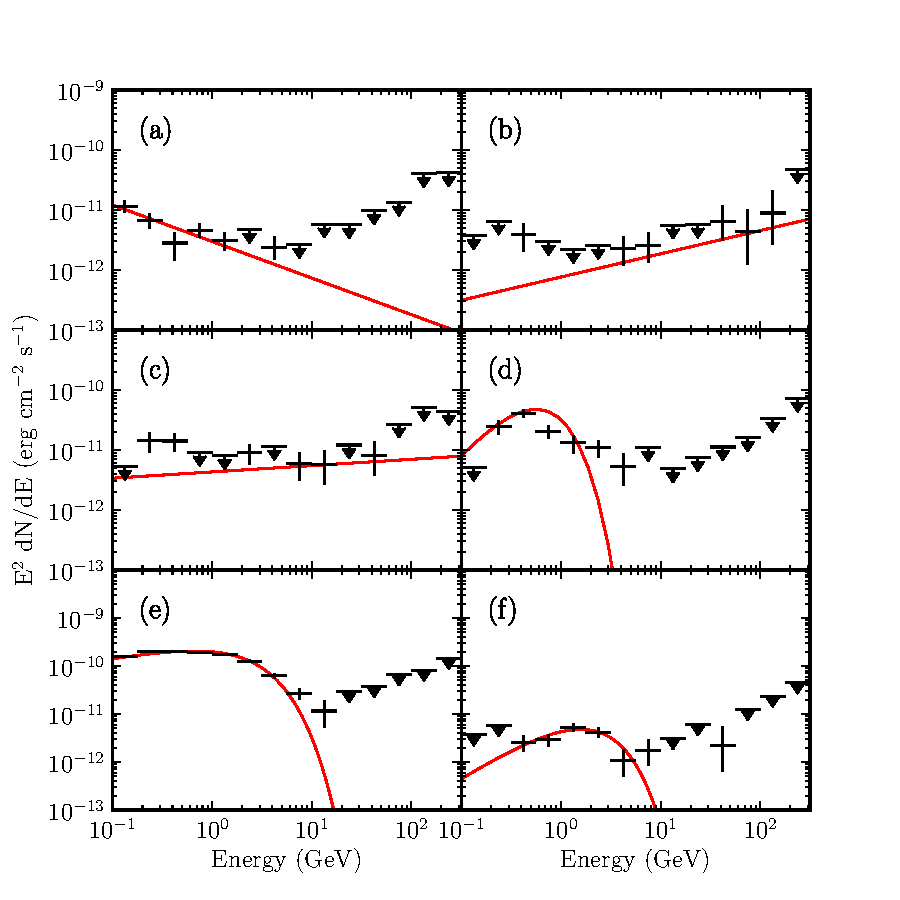
\includegraphics{chapters/offpeak/figures/off_peak_seds_color.pdf}
  \caption{Spectral energy distributions for the off-peak
  phase intervals around
  (a) PSR J0007+7303 (b) PSR J0205+6449, (c) PSR J1410$-$6132,
  (d) PSR J1747$-$2958, (e) PSR J2021+4026, and (f) PSR J2124$-$3358.
  We plot a detection in those energy bands in which the source is found with $TS\geq4$ (a $2\sigma$ detection) and report a Bayesian 95\% confidence-level upper limit otherwise.  The best-fit spectral model, using the full energy range, is also shown for comparison.
  }
  \label{off_peak_seds}
\end{figure}

\begin{figure}
  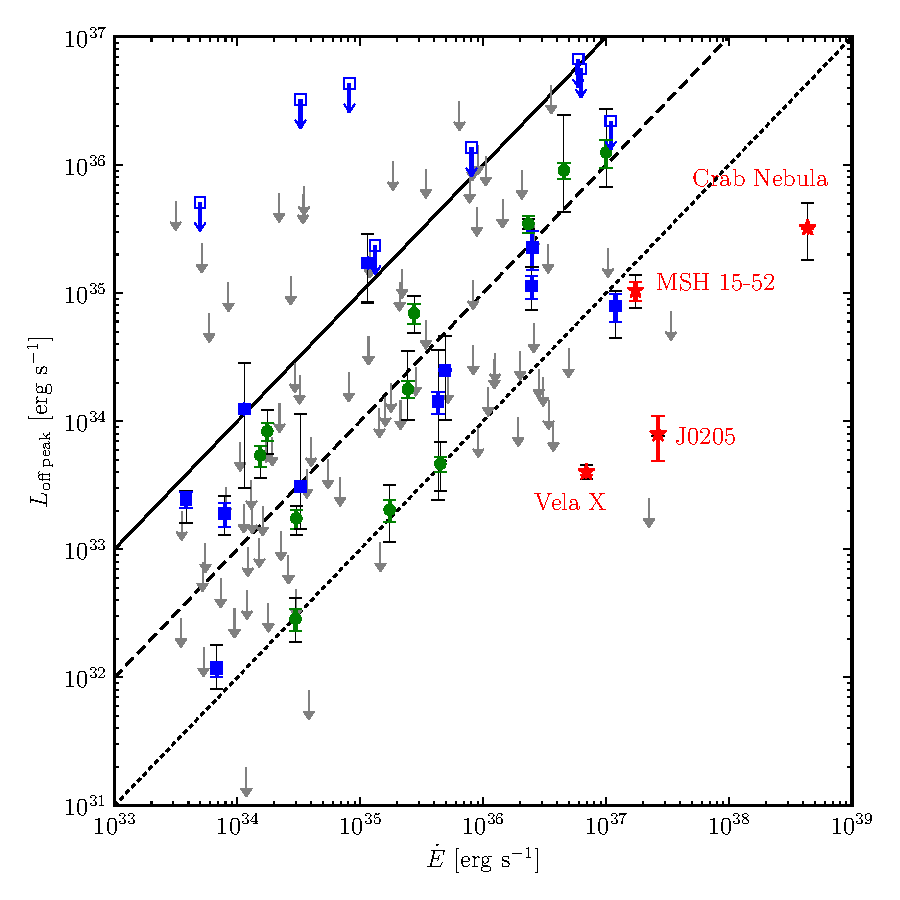
\includegraphics{chapters/offpeak/figures/off_peak_luminosity_vs_edot_color.pdf}
  \caption{The off-peak luminosity compared to the observed pulsar spindown power. 
  The luminosity is computed and plotted with the same convention as
  Figure~\ref{EDotLumG}. A luminosity upper limit is plotted
  when there is no significant off-peak emission or when there
  is only a distance upper limit.
  The
  star-shaped markers (colored red in the online version) represent
  type `W' sources, the square-shaped markers (colored blue) represent type `M' 
  and `M*' sources, 
  circular markers (colored green) represent type `U' sources,
  and the gray arrows represent non-detections.
  The filled blue square-shaped markers represent `M' and `M*' sources
  with a detected luminosity and the unfilled markers represent luminosity
  upper limits where there is only a distance upper limit.
  The solid, dashed, and dotted diagonals show 100\%, 10\%, and 1\% efficiency
  (respectively).
  }
  \figlabel{off_peak_luminosity_vs_edot}
\end{figure}

\section{Off-Peak Individual Source Discussion}
\label{off_peak_individual_source_discussion}

Here we discuss several interesting sources found in the off-peak
analysis presented in Section~\ref{unpulsed}.

% J0007+7303
The off-peak emission from PSR J0007+7303 in the SNR CTA1 was previously studied by \cite{Fermi_CTA1_2012}.
They found a soft and not-significantly cut off source in the off-peak region that
is marginally extended.
We find a similar spectrum and extension significance ($TS_{\rm ext}=10.8$), and therefore classify this
source as type `U'.


% J0205+6449
The new type `W' source is associated with PSR J0205+6449 \citep{LATPSR0205}.
The off-peak spectrum for this source is shown in panel b of Figure
\ref{off_peak_seds}.  The emission is best fit as a point source at
$(l,b)=(130\fdg73,3\fdg11)$ with a 95\% confidence-level radius of $0\fdg03$.
The source has a hard spectrum (power law with $\Gamma=1.61\pm0.21$)
and is therefore consistent with a PWN hypothesis.
This nebula has been observed at infrared
\citep{3C58_IR_PWN} and X-ray \citep{3C58_Xray_PWN} energies. This
suggests that we could be observing the inverse Compton emission from
the same electrons powering synchrotron emission at lower energies.
The PWN hypothesis is supported by the associated pulsar's
very high $\dot E=2.6\times10^{36}$ erg s$^{-1}$ and relatively young
characteristic age, $\tau_c = 5400$ yr. This is consistent with the properties
of other pulsars with LAT-detected PWN, and we favor a PWN
interpretation.
We note that the discrepancy between our spectrum and the upper limit
quoted in \citet{LAT_collaboration_PWNCAT_2011} is mainly caused by
our expanded energy range and because the flux upper limit was computed
assuming a different spectral index.


However, we note that PSR J0205+6449 is associated to the SNR 3C58
(G130.7+3.1).  Given the 2 kpc distance estimate from Section \ref{Distances}
and the density of thermal material estimated by \cite{3C58_Xray_PWN}, we can estimate
the energetics required for the LAT emission to originate in the SNR.
Following the prescription in \cite{Gamma_Visibility_SNRs_Drury_1994},
we assume the LAT emission to be hadronic and estimate a cosmic-ray
efficiency for the SNR of $\sim10$\%, which is energetically allowed.
We therefore cannot rule out the SNR hypothesis.

No TeV detection of this source has been reported, but given the hard photon
index at GeV energies this is a good candidate for observations by
an atmospheric Cherenkov telescope. Improved spectral and spatial observations 
at TeV energies might help to uniquely classify the emission.

We obtain a flux for Vela-X which is $\sim10\%$ larger than the flux
obtained in \cite{FermiVelaX2nd}. This discrepancy is most-likey due to
assuming a different spatial model for the emission (radially-symmetric
Gaussian compared to elliptical Gaussian).

% J1023-575
PSR J1023$-$5746 is associated with the TeV PWN HESS J1023$-$575
\citep{HESS_J1023-575_HESS_Collaboration_2007}.  LAT emission from
this PWN was first reported in \citet{LAT_collaboration_PWNCAT_2011}.
Because of the dominant low-energy magnetospheric emission, we classify
this as type `M' and not as a PWN.
A phase-averaged analysis of this source for energies above 10 GeV is
reported in \citet{Rousseau2013}. 


% J1119-6127
PSR J1119$-$6127 \citep{FermiMagnetars} is associated with the TeV source HESS
J1119$-$614\footnote{The discovery of HESS J1119$-$614 was presented at the
``Supernova Remnants and Pulsar Wind Nebulae in the Chandra Era'' in
2009. See \url{http://cxc.harvard.edu/cdo/snr09/pres/DjannatiAtai\_Arache\_
v2.pdf}.}. Our off-peak analysis 
classifies this source as `U' because its spectrum is soft and not significantly
cut off. However, the SED appears to represent a cutoff spectrum at low
energy and a hard rising spectrum at high energy.  
\citet{Rousseau2013} significantly detect this PWN using the analysis procedure as described for J1023$-$575.
We are likely detecting a composite of magnetospheric emission at low energy and pulsar-wind emission
at high energy.


% J1357-6429
PSR J1357$-$6429 \citep{LAT_J1357} has an associated PWN HESS J1356$-$645 detected at
TeV energies \citep{HESS_HESS_J1356-645_2011}.  Our analysis of the off-peak regions surrounding PSR
J1357$-$6429 shows a source positionally and spectrally consistent with
HESS J1356$-$645, but with significance just below detection threshold ($TS=21.0$).  
\citet{Rousseau2013} present significant emission from this source.

% J1410-6132
The off-peak region of PSR J1410$-$6132 \citep{OBrien_2008} shows a relatively hard
spectral index of $1.90\pm0.15$, and the spectrum is not significantly
cut off.  There is no associated TeV PWN
and enough low-energy GeV emission is present to caution against a clear
PWN interpretation.  We classify this source as `U', but
further observations could reveal interesting emission.

% J2021+4026
PSR J2021+4026 is spatially coincident with the
LAT-detected and spatially extended Gamma Cygni SNR
\citep{LAT_collaboration_extended_search_2012}.  The off-peak emission
from this pulsar is consistent with an exponentially-cutoff spectrum and
is therefore classified as type `M'.  The source's marginal extension
($TS_{\rm ext}=8.7$) is likely due to some contamination from the SNR.





\chapter{Search for \acp{PWN} associated with TeV Pulsars}

\section{List of Candidates}

\section{Analysis Method}

\section{Sources Detected}


\chapter{Search for \acsp{PWN} associated with High Edot Pulsars}

\chapter{Population Study of LAT-detected \acsp{PWN}}

% and the end material

\appendix

%\include{appendix1}
%\include{appendix2}
%\include{appendix3}


% bibliography style came from 
%  http://ads.harvard.edu/pubs/bibtex/astronat/apj/apj.bst
\bibliographystyle{macros/apj}

\bibliography{lande_thesis_stanford}

\end{document}

